% ===========================================================================
\section{Introduction}
% ===========================================================================
Circuit representation models encode an And-Inverter Graph (AIG) into per-gate embeddings trained to
reflect what each gate computes and reused for testability analysis, logic synthesis, Boolean
satisfiability (SAT) solving and other tasks~\cite{DBLP:conf/dac/0019KSWY022,DBLP:conf/iccad/ShiPKLLHZYCX23,DBLP:conf/iccad/ShiZKZ0024,DBLP:conf/iclr/ZhengHZSDX025,DBLP:conf/dac/WangBHZXHYH22,DBLP:conf/iccad/0006ZZLY024,DBLP:conf/dac/DengYYSCJZ24,DBLP:conf/dac/FangLLLZX25,DBLP:journals/trets/ZhaoGZWLJ26,DBLP:conf/iccad/ShiMZZPJYYCX25,DBLP:journals/corr/abs-2504-03711}.
Such reuse rests on one premise: an embedding describes the \emph{function} of a gate, not the structure
that implements it.

\begin{figure*}[t]
\centering
\mainonly{\scalebox{0.872}{\begin{tikzpicture}[x=1cm,y=1cm, font=\FB, >={Stealth[length=3.4pt]},
  ztitle/.style={font=\FT, text=ink, anchor=north west},
  zsub/.style={font=\FS, text=ink2, anchor=north west},
  ccap/.style={font=\FB, text=ink, anchor=north},
  ccap2/.style={font=\FS, text=ink2, anchor=north},
  card/.style={draw=edge, fill=white, rounded corners=2.5pt, line width=0.55pt},
  ghost/.style={draw=edge, fill=panel, rounded corners=2.5pt, line width=0.55pt},
  badge/.style={rounded corners=1.8pt, inner sep=2.4pt, font=\FK, text=white}]
\useasboundingbox (0,0) rectangle (18.00,4.95);
\draw[edge, line width=0.5pt] (7.23,0.08) -- (7.23,4.65);
\draw[edge, line width=0.5pt] (11.29,0.08) -- (11.29,4.65);
\node[ztitle] (tta) at (0.41,4.88) {One function, many certified implementations};
\node[fill=ink, text=white, font=\FK, rounded corners=1.75pt, inner sep=1.54pt, anchor=base west] at ([xshift=-10.6pt]tta.base west) {a};
\node[zsub] at (0.04,4.52) {equal numbers: SAT-proven equivalent gates; gray: none in \textit{G}};
\node[ztitle] (ttb) at (7.77,4.88) {The \emph{prediction} moves};
\node[fill=ink, text=white, font=\FK, rounded corners=1.75pt, inner sep=1.54pt, anchor=base west] at ([xshift=-10.6pt]ttb.base west) {b};
\node[zsub] at (7.40,4.52) {same function, two answers};
\node[ztitle] (ttc) at (11.83,4.88) {The \emph{representation} moves};
\node[fill=ink, text=white, font=\FK, rounded corners=1.75pt, inner sep=1.54pt, anchor=base west] at ([xshift=-10.6pt]ttc.base west) {c};
\node[zsub] at (11.46,4.52) {gates of \textit{G} ranked by cosine similarity to \textit{u}; ring: \textit{v}};
\node[ghost, minimum width=3.130cm, minimum height=3.080cm] at (5.425,2.560) {};
\node[ghost, minimum width=3.130cm, minimum height=3.080cm] at (5.295,2.460) {};
\node[ghost, minimum width=3.130cm, minimum height=3.080cm] at (5.165,2.360) {};
\node[card, minimum width=2.950cm, minimum height=2.000cm] at (1.695,1.720) {};
\node[card, minimum width=3.130cm, minimum height=3.080cm] at (5.035,2.260) {};
\draw[ink2, line width=0.5pt, -{Stealth[length=2.6pt,width=2.4pt]}] (0.9394,1.0800) -- (1.0307,1.2443);
\draw[ink2, line width=0.5pt, -{Stealth[length=2.6pt,width=2.4pt]}] (1.2506,1.0800) -- (1.1593,1.2443);
\draw[ink2, line width=0.5pt, dash pattern=on 3.112pt off 2.075pt, -{Stealth[length=2.6pt,width=2.4pt]}] (1.1705,1.4687) -- (1.2695,1.6113);
\draw[ink2, line width=0.5pt, dash pattern=on 3.346pt off 2.230pt, -{Stealth[length=2.6pt,width=2.4pt]}] (1.6561,1.0800) -- (1.4028,1.6010);
\draw[ink2, line width=0.5pt, dash pattern=on 3.357pt off 2.238pt, -{Stealth[length=2.6pt,width=2.4pt]}] (2.0506,1.0800) -- (1.9593,1.2443);
\draw[ink2, line width=0.5pt, dash pattern=on 2.747pt off 1.831pt, -{Stealth[length=2.6pt,width=2.4pt]}] (2.4150,1.0480) -- (2.0084,1.2919);
\draw[ink2, line width=0.5pt, -{Stealth[length=2.6pt,width=2.4pt]}] (2.1394,1.0800) -- (2.2307,1.2443);
\draw[ink2, line width=0.5pt, -{Stealth[length=2.6pt,width=2.4pt]}] (2.4506,1.0800) -- (2.3593,1.2443);
\draw[ink2, line width=0.5pt, dash pattern=on 3.112pt off 2.075pt, -{Stealth[length=2.6pt,width=2.4pt]}] (1.4205,1.8287) -- (1.5195,1.9713);
\draw[ink2, line width=0.5pt, dash pattern=on 2.982pt off 1.988pt, -{Stealth[length=2.6pt,width=2.4pt]}] (1.8441,1.4821) -- (1.6459,1.9579);
\draw[ink2, line width=0.5pt, dash pattern=on 3.121pt off 2.080pt, -{Stealth[length=2.6pt,width=2.4pt]}] (2.2441,1.4821) -- (1.8959,2.3179);
\draw[ink2, line width=0.5pt, dash pattern=on 3.112pt off 2.075pt, -{Stealth[length=2.6pt,width=2.4pt]}] (1.6705,2.1887) -- (1.7695,2.3313);
\fill[ink2] (1.2150,0.9200) rectangle (1.3750,1.0800);
\fill[ink2] (0.8150,0.9200) rectangle (0.9750,1.0800);
\fill[ink2] (2.0150,0.9200) rectangle (2.1750,1.0800);
\fill[ink2] (2.4150,0.9200) rectangle (2.5750,1.0800);
\fill[ink2] (1.6150,0.9200) rectangle (1.7750,1.0800);
\filldraw[fill=white, draw=ink, line width=0.7pt] (1.0950,1.3600) circle (0.1200cm);
\node[font=\FD, text=ink, inner sep=0] at (1.0950,1.3550) {1};
\filldraw[fill=white, draw=ink, line width=0.7pt] (1.3450,1.7200) circle (0.1200cm);
\node[font=\FD, text=ink, inner sep=0] at (1.3450,1.7150) {2};
\filldraw[fill=white, draw=ink, line width=0.7pt] (1.8950,1.3600) circle (0.1200cm);
\node[font=\FD, text=ink, inner sep=0] at (1.8950,1.3550) {3};
\filldraw[fill=white, draw=ink, line width=0.7pt] (2.2950,1.3600) circle (0.1200cm);
\node[font=\FD, text=ink, inner sep=0] at (2.2950,1.3550) {4};
\filldraw[fill=white, draw=ink, line width=0.7pt] (1.5950,2.0800) circle (0.1200cm);
\node[font=\FD, text=ink, inner sep=0] at (1.5950,2.0750) {5};
\filldraw[fill=ink, draw=ink, line width=0.7pt] (1.8450,2.4400) circle (0.1200cm);
\node[font=\FD, text=white, inner sep=0] at (1.8450,2.4350) {6};
\draw[ink2, line width=0.5pt, -{Stealth[length=2.6pt,width=2.4pt]}] (4.5656,1.0800) -- (4.4743,1.2443);
\draw[ink2, line width=0.5pt, -{Stealth[length=2.6pt,width=2.4pt]}] (4.2156,1.0800) -- (4.3345,1.2513);
\draw[ink2, line width=0.5pt, -{Stealth[length=2.6pt,width=2.4pt]}] (3.8044,1.0800) -- (3.7669,1.6200);
\draw[ink2, line width=0.5pt, -{Stealth[length=2.6pt,width=2.4pt]}] (4.2943,1.4241) -- (3.8477,1.6714);
\draw[ink2, line width=0.5pt, dash pattern=on 2.646pt off 1.764pt, -{Stealth[length=2.6pt,width=2.4pt]}] (3.8489,1.0800) -- (4.1162,1.6298);
\draw[ink2, line width=0.5pt, -{Stealth[length=2.6pt,width=2.4pt]}] (4.3345,1.4687) -- (4.2172,1.6377);
\draw[ink2, line width=0.5pt, dash pattern=on 3.208pt off 2.138pt, -{Stealth[length=2.6pt,width=2.4pt]}] (3.8087,1.8076) -- (3.8957,1.9643);
\draw[ink2, line width=0.5pt, dash pattern=on 3.208pt off 2.138pt, -{Stealth[length=2.6pt,width=2.4pt]}] (4.1113,1.8076) -- (4.0243,1.9643);
\draw[ink2, line width=0.5pt, -{Stealth[length=2.6pt,width=2.4pt]}] (5.5900,1.0480) -- (5.9966,1.2919);
\draw[ink2, line width=0.5pt, -{Stealth[length=2.6pt,width=2.4pt]}] (5.9544,1.0800) -- (6.0457,1.2443);
\draw[ink2, line width=0.5pt, dash pattern=on 3.282pt off 2.188pt, -{Stealth[length=2.6pt,width=2.4pt]}] (5.0378,1.0800) -- (5.5678,1.6251);
\draw[ink2, line width=0.5pt, dash pattern=on 2.734pt off 1.823pt, -{Stealth[length=2.6pt,width=2.4pt]}] (6.0067,1.4426) -- (5.7633,1.6374);
\draw[ink2, line width=0.5pt, -{Stealth[length=2.6pt,width=2.4pt]}] (5.0400,1.0427) -- (6.2215,1.6728);
\draw[ink2, line width=0.5pt, -{Stealth[length=2.6pt,width=2.4pt]}] (6.1743,1.4757) -- (6.2613,1.6324);
\draw[ink2, line width=0.5pt, -{Stealth[length=2.6pt,width=2.4pt]}] (5.5845,1.8287) -- (5.4855,1.9713);
\draw[ink2, line width=0.5pt, dash pattern=on 3.181pt off 2.121pt, -{Stealth[length=2.6pt,width=2.4pt]}] (6.2169,1.7572) -- (5.5328,2.0309);
\draw[ink2, line width=0.5pt, dash pattern=on 3.708pt off 2.472pt, -{Stealth[length=2.6pt,width=2.4pt]}] (4.6656,1.0800) -- (4.7845,1.2513);
\draw[ink2, line width=0.5pt, dash pattern=on 3.264pt off 2.176pt, -{Stealth[length=2.6pt,width=2.4pt]}] (4.2400,1.0411) -- (4.7423,1.2995);
\draw[ink2, line width=0.5pt, dash pattern=on 3.023pt off 2.015pt, -{Stealth[length=2.6pt,width=2.4pt]}] (4.5277,1.4205) -- (4.9923,1.6595);
\draw[ink2, line width=0.5pt, -{Stealth[length=2.6pt,width=2.4pt]}] (4.9355,1.4687) -- (5.0345,1.6113);
\draw[ink2, line width=0.5pt, dash pattern=on 3.112pt off 2.075pt, -{Stealth[length=2.6pt,width=2.4pt]}] (5.3345,2.1887) -- (5.2355,2.3313);
\draw[ink2, line width=0.5pt, dash pattern=on 2.650pt off 1.767pt, -{Stealth[length=2.6pt,width=2.4pt]}] (5.1192,1.8520) -- (5.1508,2.3080);
\draw[ink2, line width=0.5pt, -{Stealth[length=2.6pt,width=2.4pt]}] (4.0785,2.1388) -- (5.2915,2.7412);
\draw[ink2, line width=0.5pt, dash pattern=on 3.112pt off 2.075pt, -{Stealth[length=2.6pt,width=2.4pt]}] (5.2355,2.5487) -- (5.3345,2.6913);
\draw[ink2, line width=0.5pt, dash pattern=on 3.299pt off 2.199pt, -{Stealth[length=2.6pt,width=2.4pt]}] (4.0156,2.2001) -- (4.4179,3.0690);
\draw[ink2, line width=0.5pt, -{Stealth[length=2.6pt,width=2.4pt]}] (5.2863,2.8469) -- (4.5537,3.1245);
\draw[ink2, line width=0.5pt, -{Stealth[length=2.6pt,width=2.4pt]}] (5.3457,2.9157) -- (5.0743,3.4043);
\draw[ink2, line width=0.5pt, dash pattern=on 3.700pt off 2.466pt, -{Stealth[length=2.6pt,width=2.4pt]}] (4.5439,3.2149) -- (4.8993,3.4475);
\fill[ink2] (5.8300,0.9200) rectangle (5.9900,1.0800);
\fill[ink2] (5.4300,0.9200) rectangle (5.5900,1.0800);
\fill[ink2] (4.5300,0.9200) rectangle (4.6900,1.0800);
\fill[ink2] (4.0800,0.9200) rectangle (4.2400,1.0800);
\fill[ink2] (3.7300,0.9200) rectangle (3.8900,1.0800);
\fill[ink2] (4.8800,0.9200) rectangle (5.0400,1.0800);
\filldraw[fill=white, draw=ink, line width=0.7pt] (4.4100,1.3600) circle (0.1200cm);
\node[font=\FD, text=ink, inner sep=0] at (4.4100,1.3550) {4};
\filldraw[fill=edge, draw=rule, line width=0.6pt] (3.7600,1.7200) circle (0.0897cm);
\filldraw[fill=edge, draw=rule, line width=0.6pt] (4.1600,1.7200) circle (0.0897cm);
\filldraw[fill=white, draw=ink, line width=0.7pt, dash pattern=on 3.218pt off 2.145pt] (3.9600,2.0800) circle (0.1200cm);
\node[font=\FD, text=ink, inner sep=0] at (3.9600,2.0750) {4};
\filldraw[fill=white, draw=ink, line width=0.7pt] (6.1100,1.3600) circle (0.1200cm);
\node[font=\FD, text=ink, inner sep=0] at (6.1100,1.3550) {1};
\filldraw[fill=white, draw=ink, line width=0.7pt] (5.6600,1.7200) circle (0.1200cm);
\node[font=\FD, text=ink, inner sep=0] at (5.6600,1.7150) {2};
\filldraw[fill=edge, draw=rule, line width=0.6pt] (6.3100,1.7200) circle (0.0897cm);
\filldraw[fill=white, draw=ink, line width=0.7pt] (5.4100,2.0800) circle (0.1200cm);
\node[font=\FD, text=ink, inner sep=0] at (5.4100,2.0750) {2};
\filldraw[fill=white, draw=ink, line width=0.7pt] (4.8600,1.3600) circle (0.1200cm);
\node[font=\FD, text=ink, inner sep=0] at (4.8600,1.3550) {3};
\filldraw[fill=white, draw=ink, line width=0.7pt] (5.1100,1.7200) circle (0.1200cm);
\node[font=\FD, text=ink, inner sep=0] at (5.1100,1.7150) {3};
\filldraw[fill=white, draw=ink, line width=0.7pt] (5.1600,2.4400) circle (0.1200cm);
\node[font=\FD, text=ink, inner sep=0] at (5.1600,2.4350) {5};
\filldraw[fill=white, draw=ink, line width=0.7pt] (5.4100,2.8000) circle (0.1200cm);
\node[font=\FD, text=ink, inner sep=0] at (5.4100,2.7950) {6};
\filldraw[fill=edge, draw=rule, line width=0.6pt] (4.4600,3.1600) circle (0.0897cm);
\filldraw[fill=ink, draw=ink, line width=0.7pt] (5.0100,3.5200) circle (0.1200cm);
\node[font=\FD, text=white, inner sep=0] at (5.0100,3.5150) {6};
\node[ccap] at (1.695,0.640) {cone of \textit{v} in \textit{G}, 6 gates};
\node[ccap2] at (1.695,0.340) {\textit{G} itself has 122 gates};
\node[ccap] at (5.035,0.640) {cone of \textit{u} in \textit{G}$'$ (I.3), 14 gates};
\node[ccap2] at (5.035,0.340) {one of \NTotalVar\ certified variants};
\node[font=\FA, text=ink, anchor=east, inner sep=1.5pt] at (1.725,2.440) {\textit{v}};
\node[font=\FA, text=ink, anchor=west, inner sep=1.5pt] at (5.130,3.520) {\textit{u}};
\draw[<->, >={Stealth[length=2.8pt]}, draw=ink, line width=0.65pt, dash pattern=on 3.063pt off 2.042pt] (1.8450,2.5723) -- (1.8450,3.1700) arc[start angle=180, end angle=90, radius=0.350cm] -- (4.8777,3.5200);
\node[font=\FB, text=ink, anchor=south west, inner sep=2pt] at (0.220,3.540) {SAT proof: \textit{f}\textsubscript{\textit{v}} = \textit{f}\rlap{$'$}\textsubscript{\textit{u}}};
\draw[edge, line width=0.5pt] (7.980,1.020) -- (10.860,1.020);
\draw[edge, line width=0.5pt] (8.289,1.020) -- (8.289,0.900);
\draw[edge, line width=0.5pt] (8.803,1.020) -- (8.803,0.900);
\draw[edge, line width=0.5pt] (9.317,1.020) -- (9.317,0.900);
\draw[edge, line width=0.5pt] (9.831,1.020) -- (9.831,0.900);
\draw[edge, line width=0.5pt] (10.346,1.020) -- (10.346,0.900);
\draw[edge, line width=0.5pt] (10.860,1.020) -- (10.860,0.900);
\node[font=\FB, text=ink2, anchor=north, inner sep=1.5pt] at (8.289,0.900) {0.25};
\node[font=\FB, text=ink2, anchor=north, inner sep=1.5pt] at (9.317,0.900) {0.35};
\node[font=\FB, text=ink2, anchor=north, inner sep=1.5pt] at (10.346,0.900) {0.45};
\node[font=\FX, text=ink, anchor=north] at (9.420,0.470) {predicted \ooalign{\textit{p}\cr\hidewidth\raisebox{-0.25ex}{\kern0.12em\^{}}\hidewidth\cr}};
\draw[ink, line width=0.7pt, densely dotted] (10.343,1.020) -- (10.343,3.760);
\node[font=\FB, text=ink, anchor=south, inner sep=2pt] at (10.343,3.760) {true \textit{p}};
\node[badge, fill=cbase, anchor=north west] at (7.980,3.800) {Baseline};
\draw[cbase, line width=2.8pt, line cap=round] (8.369,3.020) -- (10.056,3.020);
\node[font=\FA, text=ink, anchor=south, inner sep=4.5pt] at (9.213,3.020) {moves 0.16};
\filldraw[fill=white, draw=cbase, line width=1.1pt] (8.369,3.020) circle (2.8pt);
\fill[cbase] (10.056,3.020) circle (2.2pt);
\node[badge, fill=cours, anchor=north west] at (7.980,2.640) {EqAlign};
\draw[cours, line width=2.8pt, line cap=round] (9.447,1.860) -- (9.867,1.860);
\node[font=\FA, text=ink, anchor=east, inner sep=6pt] at (9.447,1.860) {moves 0.04};
\filldraw[fill=white, draw=cours, line width=1.1pt] (9.447,1.860) circle (2.8pt);
\fill[cours] (9.867,1.860) circle (2.2pt);
\fill[ink] (8.060,1.460) circle (2.2pt);
\node[font=\FB, text=ink, anchor=west, inner sep=0] at (8.200,1.460) {on \textit{G}};
\filldraw[fill=white, draw=ink, line width=1.0pt] (9.200,1.460) circle (2.6pt);
\node[font=\FB, text=ink, anchor=west, inner sep=0] at (9.380,1.460) {on \textit{G}$'$};
\draw[edge, line width=0.4pt] (12.440,2.580) -- (17.780,2.580);
\node[font=\FB, text=ink2, anchor=east, inner sep=5pt] at (12.440,2.580) {0};
\draw[edge, line width=0.4pt] (12.440,2.980) -- (17.780,2.980);
\node[font=\FB, text=ink2, anchor=east, inner sep=5pt] at (12.440,2.980) {0.5};
\fill[cbase, opacity=0.10] (12.440,2.300) -- plot coordinates {(12.440,3.327) (12.484,3.257) (12.528,3.257) (12.572,3.257) (12.617,3.257) (12.661,3.257) (12.705,3.257) (12.749,3.257) (12.793,3.257) (12.837,3.257) (12.881,3.257) (12.925,3.257) (12.970,3.257) (13.014,3.257) (13.058,3.257) (13.102,3.257) (13.146,3.257) (13.190,3.257) (13.234,3.257) (13.279,3.257) (13.323,3.257) (13.367,3.257) (13.411,3.257) (13.455,3.257) (13.499,3.257) (13.543,3.257) (13.587,3.257) (13.632,3.257) (13.676,3.257) (13.720,3.257) (13.764,3.257) (13.808,3.250) (13.852,3.250) (13.896,3.250) (13.940,3.250) (13.985,3.250) (14.029,3.250) (14.073,3.250) (14.117,3.250) (14.161,3.250) (14.205,3.250) (14.249,3.250) (14.294,3.250) (14.338,3.250) (14.382,3.250) (14.426,3.250) (14.470,3.250) (14.514,3.250) (14.558,3.250) (14.602,3.250) (14.647,3.250) (14.691,3.250) (14.735,3.250) (14.779,3.250) (14.823,3.250) (14.867,3.250) (14.911,3.250) (14.956,3.250) (15.000,3.250) (15.044,3.250) (15.088,3.250) (15.132,3.250) (15.176,3.227) (15.220,3.205) (15.264,3.186) (15.309,3.181) (15.353,3.179) (15.397,3.178) (15.441,3.178) (15.485,3.178) (15.529,3.178) (15.573,3.178) (15.618,3.178) (15.662,3.178) (15.706,3.178) (15.750,3.178) (15.794,3.178) (15.838,3.178) (15.882,3.178) (15.926,3.178) (15.971,3.178) (16.015,3.178) (16.059,3.178) (16.103,3.178) (16.147,3.178) (16.191,3.178) (16.235,3.178) (16.280,3.178) (16.324,3.178) (16.368,3.178) (16.412,3.178) (16.456,3.178) (16.500,3.172) (16.544,3.172) (16.588,3.172) (16.633,3.172) (16.677,3.172) (16.721,3.172) (16.765,3.172) (16.809,3.172) (16.853,3.172) (16.897,3.172) (16.941,3.172) (16.986,3.172) (17.030,3.172) (17.074,3.172) (17.118,3.172) (17.162,3.172) (17.206,3.172) (17.250,3.172) (17.295,3.172) (17.339,3.172) (17.383,3.172) (17.427,3.172) (17.471,3.172) (17.515,3.172) (17.559,3.171) (17.603,3.170) (17.648,3.168) (17.692,3.157) (17.736,3.117) (17.780,2.792)} -- (17.780,2.300) -- cycle;
\draw[cbase, line width=1.2pt, line join=round] plot coordinates {(12.440,3.327) (12.484,3.257) (12.528,3.257) (12.572,3.257) (12.617,3.257) (12.661,3.257) (12.705,3.257) (12.749,3.257) (12.793,3.257) (12.837,3.257) (12.881,3.257) (12.925,3.257) (12.970,3.257) (13.014,3.257) (13.058,3.257) (13.102,3.257) (13.146,3.257) (13.190,3.257) (13.234,3.257) (13.279,3.257) (13.323,3.257) (13.367,3.257) (13.411,3.257) (13.455,3.257) (13.499,3.257) (13.543,3.257) (13.587,3.257) (13.632,3.257) (13.676,3.257) (13.720,3.257) (13.764,3.257) (13.808,3.250) (13.852,3.250) (13.896,3.250) (13.940,3.250) (13.985,3.250) (14.029,3.250) (14.073,3.250) (14.117,3.250) (14.161,3.250) (14.205,3.250) (14.249,3.250) (14.294,3.250) (14.338,3.250) (14.382,3.250) (14.426,3.250) (14.470,3.250) (14.514,3.250) (14.558,3.250) (14.602,3.250) (14.647,3.250) (14.691,3.250) (14.735,3.250) (14.779,3.250) (14.823,3.250) (14.867,3.250) (14.911,3.250) (14.956,3.250) (15.000,3.250) (15.044,3.250) (15.088,3.250) (15.132,3.250) (15.176,3.227) (15.220,3.205) (15.264,3.186) (15.309,3.181) (15.353,3.179) (15.397,3.178) (15.441,3.178) (15.485,3.178) (15.529,3.178) (15.573,3.178) (15.618,3.178) (15.662,3.178) (15.706,3.178) (15.750,3.178) (15.794,3.178) (15.838,3.178) (15.882,3.178) (15.926,3.178) (15.971,3.178) (16.015,3.178) (16.059,3.178) (16.103,3.178) (16.147,3.178) (16.191,3.178) (16.235,3.178) (16.280,3.178) (16.324,3.178) (16.368,3.178) (16.412,3.178) (16.456,3.178) (16.500,3.172) (16.544,3.172) (16.588,3.172) (16.633,3.172) (16.677,3.172) (16.721,3.172) (16.765,3.172) (16.809,3.172) (16.853,3.172) (16.897,3.172) (16.941,3.172) (16.986,3.172) (17.030,3.172) (17.074,3.172) (17.118,3.172) (17.162,3.172) (17.206,3.172) (17.250,3.172) (17.295,3.172) (17.339,3.172) (17.383,3.172) (17.427,3.172) (17.471,3.172) (17.515,3.172) (17.559,3.171) (17.603,3.170) (17.648,3.168) (17.692,3.157) (17.736,3.117) (17.780,2.792)};
\draw[rule, line width=0.5pt] (12.440,2.300) -- (17.780,2.300);
\draw[cbase, line width=0.6pt, densely dotted] (15.220,2.300) -- (15.220,3.205);
\filldraw[fill=white, draw=cbase, line width=1.2pt] (15.220,3.205) circle (3.0pt);
\fill[cbase] (15.220,3.205) circle (1.4pt);
\draw[ink, line width=0.6pt] (12.440,3.410) -- (12.440,3.480) -- (15.176,3.480) -- (15.176,3.410);
\node[font=\FB, text=ink, anchor=south, inner sep=1.5pt] at (13.808,3.480) {63 gates nearer to \textit{u} than \textit{v}};
\node[font=\FA, text=ink, anchor=west, inner sep=3pt] at (15.220,2.780) {rank 64};
\node[badge, fill=cbase, anchor=south east] at (17.640,2.360) {Baseline};
\draw[edge, line width=0.4pt] (12.440,1.260) -- (17.780,1.260);
\node[font=\FB, text=ink2, anchor=east, inner sep=5pt] at (12.440,1.260) {0};
\draw[edge, line width=0.4pt] (12.440,1.660) -- (17.780,1.660);
\node[font=\FB, text=ink2, anchor=east, inner sep=5pt] at (12.440,1.660) {0.5};
\fill[cours, opacity=0.10] (12.440,0.980) -- plot coordinates {(12.440,1.830) (12.484,1.566) (12.528,1.547) (12.572,1.407) (12.617,1.360) (12.661,1.319) (12.705,1.290) (12.749,1.241) (12.793,1.216) (12.837,1.216) (12.881,1.216) (12.925,1.216) (12.970,1.216) (13.014,1.216) (13.058,1.216) (13.102,1.216) (13.146,1.216) (13.190,1.216) (13.234,1.216) (13.279,1.216) (13.323,1.216) (13.367,1.216) (13.411,1.216) (13.455,1.216) (13.499,1.216) (13.543,1.216) (13.587,1.216) (13.632,1.216) (13.676,1.216) (13.720,1.216) (13.764,1.216) (13.808,1.216) (13.852,1.216) (13.896,1.216) (13.940,1.216) (13.985,1.216) (14.029,1.216) (14.073,1.216) (14.117,1.184) (14.161,1.176) (14.205,1.163) (14.249,1.160) (14.294,1.155) (14.338,1.140) (14.382,1.138) (14.426,1.131) (14.470,1.112) (14.514,1.111) (14.558,1.111) (14.602,1.111) (14.647,1.111) (14.691,1.111) (14.735,1.111) (14.779,1.111) (14.823,1.111) (14.867,1.111) (14.911,1.111) (14.956,1.111) (15.000,1.111) (15.044,1.111) (15.088,1.111) (15.132,1.111) (15.176,1.111) (15.220,1.111) (15.264,1.111) (15.309,1.111) (15.353,1.111) (15.397,1.111) (15.441,1.111) (15.485,1.111) (15.529,1.111) (15.573,1.111) (15.618,1.111) (15.662,1.111) (15.706,1.111) (15.750,1.111) (15.794,1.111) (15.838,1.111) (15.882,1.105) (15.926,1.086) (15.971,1.081) (16.015,1.073) (16.059,1.069) (16.103,1.064) (16.147,1.059) (16.191,1.054) (16.235,1.052) (16.280,1.052) (16.324,1.050) (16.368,1.050) (16.412,1.050) (16.456,1.050) (16.500,1.050) (16.544,1.050) (16.588,1.050) (16.633,1.050) (16.677,1.050) (16.721,1.050) (16.765,1.050) (16.809,1.050) (16.853,1.049) (16.897,1.049) (16.941,1.049) (16.986,1.049) (17.030,1.049) (17.074,1.047) (17.118,1.045) (17.162,1.045) (17.206,1.045) (17.250,1.045) (17.295,1.045) (17.339,1.045) (17.383,1.045) (17.427,1.045) (17.471,1.045) (17.515,1.045) (17.559,1.045) (17.603,1.045) (17.648,1.045) (17.692,1.045) (17.736,1.045) (17.780,1.045)} -- (17.780,0.980) -- cycle;
\draw[cours, line width=1.2pt, line join=round] plot coordinates {(12.440,1.830) (12.484,1.566) (12.528,1.547) (12.572,1.407) (12.617,1.360) (12.661,1.319) (12.705,1.290) (12.749,1.241) (12.793,1.216) (12.837,1.216) (12.881,1.216) (12.925,1.216) (12.970,1.216) (13.014,1.216) (13.058,1.216) (13.102,1.216) (13.146,1.216) (13.190,1.216) (13.234,1.216) (13.279,1.216) (13.323,1.216) (13.367,1.216) (13.411,1.216) (13.455,1.216) (13.499,1.216) (13.543,1.216) (13.587,1.216) (13.632,1.216) (13.676,1.216) (13.720,1.216) (13.764,1.216) (13.808,1.216) (13.852,1.216) (13.896,1.216) (13.940,1.216) (13.985,1.216) (14.029,1.216) (14.073,1.216) (14.117,1.184) (14.161,1.176) (14.205,1.163) (14.249,1.160) (14.294,1.155) (14.338,1.140) (14.382,1.138) (14.426,1.131) (14.470,1.112) (14.514,1.111) (14.558,1.111) (14.602,1.111) (14.647,1.111) (14.691,1.111) (14.735,1.111) (14.779,1.111) (14.823,1.111) (14.867,1.111) (14.911,1.111) (14.956,1.111) (15.000,1.111) (15.044,1.111) (15.088,1.111) (15.132,1.111) (15.176,1.111) (15.220,1.111) (15.264,1.111) (15.309,1.111) (15.353,1.111) (15.397,1.111) (15.441,1.111) (15.485,1.111) (15.529,1.111) (15.573,1.111) (15.618,1.111) (15.662,1.111) (15.706,1.111) (15.750,1.111) (15.794,1.111) (15.838,1.111) (15.882,1.105) (15.926,1.086) (15.971,1.081) (16.015,1.073) (16.059,1.069) (16.103,1.064) (16.147,1.059) (16.191,1.054) (16.235,1.052) (16.280,1.052) (16.324,1.050) (16.368,1.050) (16.412,1.050) (16.456,1.050) (16.500,1.050) (16.544,1.050) (16.588,1.050) (16.633,1.050) (16.677,1.050) (16.721,1.050) (16.765,1.050) (16.809,1.050) (16.853,1.049) (16.897,1.049) (16.941,1.049) (16.986,1.049) (17.030,1.049) (17.074,1.047) (17.118,1.045) (17.162,1.045) (17.206,1.045) (17.250,1.045) (17.295,1.045) (17.339,1.045) (17.383,1.045) (17.427,1.045) (17.471,1.045) (17.515,1.045) (17.559,1.045) (17.603,1.045) (17.648,1.045) (17.692,1.045) (17.736,1.045) (17.780,1.045)};
\draw[rule, line width=0.5pt] (12.440,0.980) -- (17.780,0.980);
\draw[cours, line width=0.6pt, densely dotted] (12.440,0.980) -- (12.440,1.830);
\filldraw[fill=white, draw=cours, line width=1.2pt] (12.440,1.830) circle (3.0pt);
\fill[cours] (12.440,1.830) circle (1.4pt);
\node[font=\FA, text=ink, anchor=west, inner sep=4.5pt] at (12.440,1.830) {rank 1: \textit{v} is the nearest gate};
\node[badge, fill=cours, anchor=north east] at (17.780,2.060) {EqAlign};
\draw[ink2, line width=0.5pt] (12.440,0.960) -- (12.440,0.860);
\node[font=\FB, text=ink2, anchor=north, inner sep=1.5pt] at (12.440,0.860) {1};
\draw[ink2, line width=0.5pt] (13.808,0.960) -- (13.808,0.860);
\node[font=\FB, text=ink2, anchor=north, inner sep=1.5pt] at (13.808,0.860) {32};
\draw[ink2, line width=0.5pt] (15.220,0.960) -- (15.220,0.860);
\node[font=\FB, text=ink2, anchor=north, inner sep=1.5pt] at (15.220,0.860) {64};
\draw[ink2, line width=0.5pt] (16.633,0.960) -- (16.633,0.860);
\node[font=\FB, text=ink2, anchor=north, inner sep=1.5pt] at (16.633,0.860) {96};
\draw[ink2, line width=0.5pt] (17.780,0.960) -- (17.780,0.860);
\node[font=\FB, text=ink2, anchor=north, inner sep=1.5pt] at (17.780,0.860) {122};
\node[font=\FX, text=ink, anchor=north] at (15.110,0.540) {rank among the 122 gates of \textit{G}, most similar first};
\node[font=\FX, text=ink, rotate=90, anchor=south] at (11.920,2.180) {cosine similarity to \textbf{z}\rlap{$'$}\textsubscript{\textit{u}}};
\end{tikzpicture}
}}\extonly{\begin{tikzpicture}[x=1cm,y=1cm, font=\FB, >={Stealth[length=3.4pt]},
  ztitle/.style={font=\FT, text=ink, anchor=north west},
  zsub/.style={font=\FS, text=ink2, anchor=north west},
  ccap/.style={font=\FB, text=ink, anchor=north},
  ccap2/.style={font=\FS, text=ink2, anchor=north},
  card/.style={draw=edge, fill=white, rounded corners=2.5pt, line width=0.55pt},
  ghost/.style={draw=edge, fill=panel, rounded corners=2.5pt, line width=0.55pt},
  badge/.style={rounded corners=1.8pt, inner sep=2.4pt, font=\FK, text=white}]
\useasboundingbox (0,0) rectangle (18.00,4.95);
\draw[edge, line width=0.5pt] (7.23,0.08) -- (7.23,4.65);
\draw[edge, line width=0.5pt] (11.29,0.08) -- (11.29,4.65);
\node[ztitle] (tta) at (0.41,4.88) {One function, many certified implementations};
\node[fill=ink, text=white, font=\FK, rounded corners=1.75pt, inner sep=1.54pt, anchor=base west] at ([xshift=-10.6pt]tta.base west) {a};
\node[zsub] at (0.04,4.52) {equal numbers: SAT-proven equivalent gates; gray: none in \textit{G}};
\node[ztitle] (ttb) at (7.77,4.88) {The \emph{prediction} moves};
\node[fill=ink, text=white, font=\FK, rounded corners=1.75pt, inner sep=1.54pt, anchor=base west] at ([xshift=-10.6pt]ttb.base west) {b};
\node[zsub] at (7.40,4.52) {same function, two answers};
\node[ztitle] (ttc) at (11.83,4.88) {The \emph{representation} moves};
\node[fill=ink, text=white, font=\FK, rounded corners=1.75pt, inner sep=1.54pt, anchor=base west] at ([xshift=-10.6pt]ttc.base west) {c};
\node[zsub] at (11.46,4.52) {gates of \textit{G} ranked by cosine similarity to \textit{u}; ring: \textit{v}};
\node[ghost, minimum width=3.130cm, minimum height=3.080cm] at (5.425,2.560) {};
\node[ghost, minimum width=3.130cm, minimum height=3.080cm] at (5.295,2.460) {};
\node[ghost, minimum width=3.130cm, minimum height=3.080cm] at (5.165,2.360) {};
\node[card, minimum width=2.950cm, minimum height=2.000cm] at (1.695,1.720) {};
\node[card, minimum width=3.130cm, minimum height=3.080cm] at (5.035,2.260) {};
\draw[ink2, line width=0.5pt, -{Stealth[length=2.6pt,width=2.4pt]}] (0.9394,1.0800) -- (1.0307,1.2443);
\draw[ink2, line width=0.5pt, -{Stealth[length=2.6pt,width=2.4pt]}] (1.2506,1.0800) -- (1.1593,1.2443);
\draw[ink2, line width=0.5pt, dash pattern=on 3.112pt off 2.075pt, -{Stealth[length=2.6pt,width=2.4pt]}] (1.1705,1.4687) -- (1.2695,1.6113);
\draw[ink2, line width=0.5pt, dash pattern=on 3.346pt off 2.230pt, -{Stealth[length=2.6pt,width=2.4pt]}] (1.6561,1.0800) -- (1.4028,1.6010);
\draw[ink2, line width=0.5pt, dash pattern=on 3.357pt off 2.238pt, -{Stealth[length=2.6pt,width=2.4pt]}] (2.0506,1.0800) -- (1.9593,1.2443);
\draw[ink2, line width=0.5pt, dash pattern=on 2.747pt off 1.831pt, -{Stealth[length=2.6pt,width=2.4pt]}] (2.4150,1.0480) -- (2.0084,1.2919);
\draw[ink2, line width=0.5pt, -{Stealth[length=2.6pt,width=2.4pt]}] (2.1394,1.0800) -- (2.2307,1.2443);
\draw[ink2, line width=0.5pt, -{Stealth[length=2.6pt,width=2.4pt]}] (2.4506,1.0800) -- (2.3593,1.2443);
\draw[ink2, line width=0.5pt, dash pattern=on 3.112pt off 2.075pt, -{Stealth[length=2.6pt,width=2.4pt]}] (1.4205,1.8287) -- (1.5195,1.9713);
\draw[ink2, line width=0.5pt, dash pattern=on 2.982pt off 1.988pt, -{Stealth[length=2.6pt,width=2.4pt]}] (1.8441,1.4821) -- (1.6459,1.9579);
\draw[ink2, line width=0.5pt, dash pattern=on 3.121pt off 2.080pt, -{Stealth[length=2.6pt,width=2.4pt]}] (2.2441,1.4821) -- (1.8959,2.3179);
\draw[ink2, line width=0.5pt, dash pattern=on 3.112pt off 2.075pt, -{Stealth[length=2.6pt,width=2.4pt]}] (1.6705,2.1887) -- (1.7695,2.3313);
\fill[ink2] (1.2150,0.9200) rectangle (1.3750,1.0800);
\fill[ink2] (0.8150,0.9200) rectangle (0.9750,1.0800);
\fill[ink2] (2.0150,0.9200) rectangle (2.1750,1.0800);
\fill[ink2] (2.4150,0.9200) rectangle (2.5750,1.0800);
\fill[ink2] (1.6150,0.9200) rectangle (1.7750,1.0800);
\filldraw[fill=white, draw=ink, line width=0.7pt] (1.0950,1.3600) circle (0.1200cm);
\node[font=\FD, text=ink, inner sep=0] at (1.0950,1.3550) {1};
\filldraw[fill=white, draw=ink, line width=0.7pt] (1.3450,1.7200) circle (0.1200cm);
\node[font=\FD, text=ink, inner sep=0] at (1.3450,1.7150) {2};
\filldraw[fill=white, draw=ink, line width=0.7pt] (1.8950,1.3600) circle (0.1200cm);
\node[font=\FD, text=ink, inner sep=0] at (1.8950,1.3550) {3};
\filldraw[fill=white, draw=ink, line width=0.7pt] (2.2950,1.3600) circle (0.1200cm);
\node[font=\FD, text=ink, inner sep=0] at (2.2950,1.3550) {4};
\filldraw[fill=white, draw=ink, line width=0.7pt] (1.5950,2.0800) circle (0.1200cm);
\node[font=\FD, text=ink, inner sep=0] at (1.5950,2.0750) {5};
\filldraw[fill=ink, draw=ink, line width=0.7pt] (1.8450,2.4400) circle (0.1200cm);
\node[font=\FD, text=white, inner sep=0] at (1.8450,2.4350) {6};
\draw[ink2, line width=0.5pt, -{Stealth[length=2.6pt,width=2.4pt]}] (4.5656,1.0800) -- (4.4743,1.2443);
\draw[ink2, line width=0.5pt, -{Stealth[length=2.6pt,width=2.4pt]}] (4.2156,1.0800) -- (4.3345,1.2513);
\draw[ink2, line width=0.5pt, -{Stealth[length=2.6pt,width=2.4pt]}] (3.8044,1.0800) -- (3.7669,1.6200);
\draw[ink2, line width=0.5pt, -{Stealth[length=2.6pt,width=2.4pt]}] (4.2943,1.4241) -- (3.8477,1.6714);
\draw[ink2, line width=0.5pt, dash pattern=on 2.646pt off 1.764pt, -{Stealth[length=2.6pt,width=2.4pt]}] (3.8489,1.0800) -- (4.1162,1.6298);
\draw[ink2, line width=0.5pt, -{Stealth[length=2.6pt,width=2.4pt]}] (4.3345,1.4687) -- (4.2172,1.6377);
\draw[ink2, line width=0.5pt, dash pattern=on 3.208pt off 2.138pt, -{Stealth[length=2.6pt,width=2.4pt]}] (3.8087,1.8076) -- (3.8957,1.9643);
\draw[ink2, line width=0.5pt, dash pattern=on 3.208pt off 2.138pt, -{Stealth[length=2.6pt,width=2.4pt]}] (4.1113,1.8076) -- (4.0243,1.9643);
\draw[ink2, line width=0.5pt, -{Stealth[length=2.6pt,width=2.4pt]}] (5.5900,1.0480) -- (5.9966,1.2919);
\draw[ink2, line width=0.5pt, -{Stealth[length=2.6pt,width=2.4pt]}] (5.9544,1.0800) -- (6.0457,1.2443);
\draw[ink2, line width=0.5pt, dash pattern=on 3.282pt off 2.188pt, -{Stealth[length=2.6pt,width=2.4pt]}] (5.0378,1.0800) -- (5.5678,1.6251);
\draw[ink2, line width=0.5pt, dash pattern=on 2.734pt off 1.823pt, -{Stealth[length=2.6pt,width=2.4pt]}] (6.0067,1.4426) -- (5.7633,1.6374);
\draw[ink2, line width=0.5pt, -{Stealth[length=2.6pt,width=2.4pt]}] (5.0400,1.0427) -- (6.2215,1.6728);
\draw[ink2, line width=0.5pt, -{Stealth[length=2.6pt,width=2.4pt]}] (6.1743,1.4757) -- (6.2613,1.6324);
\draw[ink2, line width=0.5pt, -{Stealth[length=2.6pt,width=2.4pt]}] (5.5845,1.8287) -- (5.4855,1.9713);
\draw[ink2, line width=0.5pt, dash pattern=on 3.181pt off 2.121pt, -{Stealth[length=2.6pt,width=2.4pt]}] (6.2169,1.7572) -- (5.5328,2.0309);
\draw[ink2, line width=0.5pt, dash pattern=on 3.708pt off 2.472pt, -{Stealth[length=2.6pt,width=2.4pt]}] (4.6656,1.0800) -- (4.7845,1.2513);
\draw[ink2, line width=0.5pt, dash pattern=on 3.264pt off 2.176pt, -{Stealth[length=2.6pt,width=2.4pt]}] (4.2400,1.0411) -- (4.7423,1.2995);
\draw[ink2, line width=0.5pt, dash pattern=on 3.023pt off 2.015pt, -{Stealth[length=2.6pt,width=2.4pt]}] (4.5277,1.4205) -- (4.9923,1.6595);
\draw[ink2, line width=0.5pt, -{Stealth[length=2.6pt,width=2.4pt]}] (4.9355,1.4687) -- (5.0345,1.6113);
\draw[ink2, line width=0.5pt, dash pattern=on 3.112pt off 2.075pt, -{Stealth[length=2.6pt,width=2.4pt]}] (5.3345,2.1887) -- (5.2355,2.3313);
\draw[ink2, line width=0.5pt, dash pattern=on 2.650pt off 1.767pt, -{Stealth[length=2.6pt,width=2.4pt]}] (5.1192,1.8520) -- (5.1508,2.3080);
\draw[ink2, line width=0.5pt, -{Stealth[length=2.6pt,width=2.4pt]}] (4.0785,2.1388) -- (5.2915,2.7412);
\draw[ink2, line width=0.5pt, dash pattern=on 3.112pt off 2.075pt, -{Stealth[length=2.6pt,width=2.4pt]}] (5.2355,2.5487) -- (5.3345,2.6913);
\draw[ink2, line width=0.5pt, dash pattern=on 3.299pt off 2.199pt, -{Stealth[length=2.6pt,width=2.4pt]}] (4.0156,2.2001) -- (4.4179,3.0690);
\draw[ink2, line width=0.5pt, -{Stealth[length=2.6pt,width=2.4pt]}] (5.2863,2.8469) -- (4.5537,3.1245);
\draw[ink2, line width=0.5pt, -{Stealth[length=2.6pt,width=2.4pt]}] (5.3457,2.9157) -- (5.0743,3.4043);
\draw[ink2, line width=0.5pt, dash pattern=on 3.700pt off 2.466pt, -{Stealth[length=2.6pt,width=2.4pt]}] (4.5439,3.2149) -- (4.8993,3.4475);
\fill[ink2] (5.8300,0.9200) rectangle (5.9900,1.0800);
\fill[ink2] (5.4300,0.9200) rectangle (5.5900,1.0800);
\fill[ink2] (4.5300,0.9200) rectangle (4.6900,1.0800);
\fill[ink2] (4.0800,0.9200) rectangle (4.2400,1.0800);
\fill[ink2] (3.7300,0.9200) rectangle (3.8900,1.0800);
\fill[ink2] (4.8800,0.9200) rectangle (5.0400,1.0800);
\filldraw[fill=white, draw=ink, line width=0.7pt] (4.4100,1.3600) circle (0.1200cm);
\node[font=\FD, text=ink, inner sep=0] at (4.4100,1.3550) {4};
\filldraw[fill=edge, draw=rule, line width=0.6pt] (3.7600,1.7200) circle (0.0897cm);
\filldraw[fill=edge, draw=rule, line width=0.6pt] (4.1600,1.7200) circle (0.0897cm);
\filldraw[fill=white, draw=ink, line width=0.7pt, dash pattern=on 3.218pt off 2.145pt] (3.9600,2.0800) circle (0.1200cm);
\node[font=\FD, text=ink, inner sep=0] at (3.9600,2.0750) {4};
\filldraw[fill=white, draw=ink, line width=0.7pt] (6.1100,1.3600) circle (0.1200cm);
\node[font=\FD, text=ink, inner sep=0] at (6.1100,1.3550) {1};
\filldraw[fill=white, draw=ink, line width=0.7pt] (5.6600,1.7200) circle (0.1200cm);
\node[font=\FD, text=ink, inner sep=0] at (5.6600,1.7150) {2};
\filldraw[fill=edge, draw=rule, line width=0.6pt] (6.3100,1.7200) circle (0.0897cm);
\filldraw[fill=white, draw=ink, line width=0.7pt] (5.4100,2.0800) circle (0.1200cm);
\node[font=\FD, text=ink, inner sep=0] at (5.4100,2.0750) {2};
\filldraw[fill=white, draw=ink, line width=0.7pt] (4.8600,1.3600) circle (0.1200cm);
\node[font=\FD, text=ink, inner sep=0] at (4.8600,1.3550) {3};
\filldraw[fill=white, draw=ink, line width=0.7pt] (5.1100,1.7200) circle (0.1200cm);
\node[font=\FD, text=ink, inner sep=0] at (5.1100,1.7150) {3};
\filldraw[fill=white, draw=ink, line width=0.7pt] (5.1600,2.4400) circle (0.1200cm);
\node[font=\FD, text=ink, inner sep=0] at (5.1600,2.4350) {5};
\filldraw[fill=white, draw=ink, line width=0.7pt] (5.4100,2.8000) circle (0.1200cm);
\node[font=\FD, text=ink, inner sep=0] at (5.4100,2.7950) {6};
\filldraw[fill=edge, draw=rule, line width=0.6pt] (4.4600,3.1600) circle (0.0897cm);
\filldraw[fill=ink, draw=ink, line width=0.7pt] (5.0100,3.5200) circle (0.1200cm);
\node[font=\FD, text=white, inner sep=0] at (5.0100,3.5150) {6};
\node[ccap] at (1.695,0.640) {cone of \textit{v} in \textit{G}, 6 gates};
\node[ccap2] at (1.695,0.340) {\textit{G} itself has 122 gates};
\node[ccap] at (5.035,0.640) {cone of \textit{u} in \textit{G}$'$ (I.3), 14 gates};
\node[ccap2] at (5.035,0.340) {one of \NTotalVar\ certified variants};
\node[font=\FA, text=ink, anchor=east, inner sep=1.5pt] at (1.725,2.440) {\textit{v}};
\node[font=\FA, text=ink, anchor=west, inner sep=1.5pt] at (5.130,3.520) {\textit{u}};
\draw[<->, >={Stealth[length=2.8pt]}, draw=ink, line width=0.65pt, dash pattern=on 3.063pt off 2.042pt] (1.8450,2.5723) -- (1.8450,3.1700) arc[start angle=180, end angle=90, radius=0.350cm] -- (4.8777,3.5200);
\node[font=\FB, text=ink, anchor=south west, inner sep=2pt] at (0.220,3.540) {SAT proof: \textit{f}\textsubscript{\textit{v}} = \textit{f}\rlap{$'$}\textsubscript{\textit{u}}};
\draw[edge, line width=0.5pt] (7.980,1.020) -- (10.860,1.020);
\draw[edge, line width=0.5pt] (8.289,1.020) -- (8.289,0.900);
\draw[edge, line width=0.5pt] (8.803,1.020) -- (8.803,0.900);
\draw[edge, line width=0.5pt] (9.317,1.020) -- (9.317,0.900);
\draw[edge, line width=0.5pt] (9.831,1.020) -- (9.831,0.900);
\draw[edge, line width=0.5pt] (10.346,1.020) -- (10.346,0.900);
\draw[edge, line width=0.5pt] (10.860,1.020) -- (10.860,0.900);
\node[font=\FB, text=ink2, anchor=north, inner sep=1.5pt] at (8.289,0.900) {0.25};
\node[font=\FB, text=ink2, anchor=north, inner sep=1.5pt] at (9.317,0.900) {0.35};
\node[font=\FB, text=ink2, anchor=north, inner sep=1.5pt] at (10.346,0.900) {0.45};
\node[font=\FX, text=ink, anchor=north] at (9.420,0.470) {predicted \ooalign{\textit{p}\cr\hidewidth\raisebox{-0.25ex}{\kern0.12em\^{}}\hidewidth\cr}};
\draw[ink, line width=0.7pt, densely dotted] (10.343,1.020) -- (10.343,3.760);
\node[font=\FB, text=ink, anchor=south, inner sep=2pt] at (10.343,3.760) {true \textit{p}};
\node[badge, fill=cbase, anchor=north west] at (7.980,3.800) {Baseline};
\draw[cbase, line width=2.8pt, line cap=round] (8.369,3.020) -- (10.056,3.020);
\node[font=\FA, text=ink, anchor=south, inner sep=4.5pt] at (9.213,3.020) {moves 0.16};
\filldraw[fill=white, draw=cbase, line width=1.1pt] (8.369,3.020) circle (2.8pt);
\fill[cbase] (10.056,3.020) circle (2.2pt);
\node[badge, fill=cours, anchor=north west] at (7.980,2.640) {EqAlign};
\draw[cours, line width=2.8pt, line cap=round] (9.447,1.860) -- (9.867,1.860);
\node[font=\FA, text=ink, anchor=east, inner sep=6pt] at (9.447,1.860) {moves 0.04};
\filldraw[fill=white, draw=cours, line width=1.1pt] (9.447,1.860) circle (2.8pt);
\fill[cours] (9.867,1.860) circle (2.2pt);
\fill[ink] (8.060,1.460) circle (2.2pt);
\node[font=\FB, text=ink, anchor=west, inner sep=0] at (8.200,1.460) {on \textit{G}};
\filldraw[fill=white, draw=ink, line width=1.0pt] (9.200,1.460) circle (2.6pt);
\node[font=\FB, text=ink, anchor=west, inner sep=0] at (9.380,1.460) {on \textit{G}$'$};
\draw[edge, line width=0.4pt] (12.440,2.580) -- (17.780,2.580);
\node[font=\FB, text=ink2, anchor=east, inner sep=5pt] at (12.440,2.580) {0};
\draw[edge, line width=0.4pt] (12.440,2.980) -- (17.780,2.980);
\node[font=\FB, text=ink2, anchor=east, inner sep=5pt] at (12.440,2.980) {0.5};
\fill[cbase, opacity=0.10] (12.440,2.300) -- plot coordinates {(12.440,3.327) (12.484,3.257) (12.528,3.257) (12.572,3.257) (12.617,3.257) (12.661,3.257) (12.705,3.257) (12.749,3.257) (12.793,3.257) (12.837,3.257) (12.881,3.257) (12.925,3.257) (12.970,3.257) (13.014,3.257) (13.058,3.257) (13.102,3.257) (13.146,3.257) (13.190,3.257) (13.234,3.257) (13.279,3.257) (13.323,3.257) (13.367,3.257) (13.411,3.257) (13.455,3.257) (13.499,3.257) (13.543,3.257) (13.587,3.257) (13.632,3.257) (13.676,3.257) (13.720,3.257) (13.764,3.257) (13.808,3.250) (13.852,3.250) (13.896,3.250) (13.940,3.250) (13.985,3.250) (14.029,3.250) (14.073,3.250) (14.117,3.250) (14.161,3.250) (14.205,3.250) (14.249,3.250) (14.294,3.250) (14.338,3.250) (14.382,3.250) (14.426,3.250) (14.470,3.250) (14.514,3.250) (14.558,3.250) (14.602,3.250) (14.647,3.250) (14.691,3.250) (14.735,3.250) (14.779,3.250) (14.823,3.250) (14.867,3.250) (14.911,3.250) (14.956,3.250) (15.000,3.250) (15.044,3.250) (15.088,3.250) (15.132,3.250) (15.176,3.227) (15.220,3.205) (15.264,3.186) (15.309,3.181) (15.353,3.179) (15.397,3.178) (15.441,3.178) (15.485,3.178) (15.529,3.178) (15.573,3.178) (15.618,3.178) (15.662,3.178) (15.706,3.178) (15.750,3.178) (15.794,3.178) (15.838,3.178) (15.882,3.178) (15.926,3.178) (15.971,3.178) (16.015,3.178) (16.059,3.178) (16.103,3.178) (16.147,3.178) (16.191,3.178) (16.235,3.178) (16.280,3.178) (16.324,3.178) (16.368,3.178) (16.412,3.178) (16.456,3.178) (16.500,3.172) (16.544,3.172) (16.588,3.172) (16.633,3.172) (16.677,3.172) (16.721,3.172) (16.765,3.172) (16.809,3.172) (16.853,3.172) (16.897,3.172) (16.941,3.172) (16.986,3.172) (17.030,3.172) (17.074,3.172) (17.118,3.172) (17.162,3.172) (17.206,3.172) (17.250,3.172) (17.295,3.172) (17.339,3.172) (17.383,3.172) (17.427,3.172) (17.471,3.172) (17.515,3.172) (17.559,3.171) (17.603,3.170) (17.648,3.168) (17.692,3.157) (17.736,3.117) (17.780,2.792)} -- (17.780,2.300) -- cycle;
\draw[cbase, line width=1.2pt, line join=round] plot coordinates {(12.440,3.327) (12.484,3.257) (12.528,3.257) (12.572,3.257) (12.617,3.257) (12.661,3.257) (12.705,3.257) (12.749,3.257) (12.793,3.257) (12.837,3.257) (12.881,3.257) (12.925,3.257) (12.970,3.257) (13.014,3.257) (13.058,3.257) (13.102,3.257) (13.146,3.257) (13.190,3.257) (13.234,3.257) (13.279,3.257) (13.323,3.257) (13.367,3.257) (13.411,3.257) (13.455,3.257) (13.499,3.257) (13.543,3.257) (13.587,3.257) (13.632,3.257) (13.676,3.257) (13.720,3.257) (13.764,3.257) (13.808,3.250) (13.852,3.250) (13.896,3.250) (13.940,3.250) (13.985,3.250) (14.029,3.250) (14.073,3.250) (14.117,3.250) (14.161,3.250) (14.205,3.250) (14.249,3.250) (14.294,3.250) (14.338,3.250) (14.382,3.250) (14.426,3.250) (14.470,3.250) (14.514,3.250) (14.558,3.250) (14.602,3.250) (14.647,3.250) (14.691,3.250) (14.735,3.250) (14.779,3.250) (14.823,3.250) (14.867,3.250) (14.911,3.250) (14.956,3.250) (15.000,3.250) (15.044,3.250) (15.088,3.250) (15.132,3.250) (15.176,3.227) (15.220,3.205) (15.264,3.186) (15.309,3.181) (15.353,3.179) (15.397,3.178) (15.441,3.178) (15.485,3.178) (15.529,3.178) (15.573,3.178) (15.618,3.178) (15.662,3.178) (15.706,3.178) (15.750,3.178) (15.794,3.178) (15.838,3.178) (15.882,3.178) (15.926,3.178) (15.971,3.178) (16.015,3.178) (16.059,3.178) (16.103,3.178) (16.147,3.178) (16.191,3.178) (16.235,3.178) (16.280,3.178) (16.324,3.178) (16.368,3.178) (16.412,3.178) (16.456,3.178) (16.500,3.172) (16.544,3.172) (16.588,3.172) (16.633,3.172) (16.677,3.172) (16.721,3.172) (16.765,3.172) (16.809,3.172) (16.853,3.172) (16.897,3.172) (16.941,3.172) (16.986,3.172) (17.030,3.172) (17.074,3.172) (17.118,3.172) (17.162,3.172) (17.206,3.172) (17.250,3.172) (17.295,3.172) (17.339,3.172) (17.383,3.172) (17.427,3.172) (17.471,3.172) (17.515,3.172) (17.559,3.171) (17.603,3.170) (17.648,3.168) (17.692,3.157) (17.736,3.117) (17.780,2.792)};
\draw[rule, line width=0.5pt] (12.440,2.300) -- (17.780,2.300);
\draw[cbase, line width=0.6pt, densely dotted] (15.220,2.300) -- (15.220,3.205);
\filldraw[fill=white, draw=cbase, line width=1.2pt] (15.220,3.205) circle (3.0pt);
\fill[cbase] (15.220,3.205) circle (1.4pt);
\draw[ink, line width=0.6pt] (12.440,3.410) -- (12.440,3.480) -- (15.176,3.480) -- (15.176,3.410);
\node[font=\FB, text=ink, anchor=south, inner sep=1.5pt] at (13.808,3.480) {63 gates nearer to \textit{u} than \textit{v}};
\node[font=\FA, text=ink, anchor=west, inner sep=3pt] at (15.220,2.780) {rank 64};
\node[badge, fill=cbase, anchor=south east] at (17.640,2.360) {Baseline};
\draw[edge, line width=0.4pt] (12.440,1.260) -- (17.780,1.260);
\node[font=\FB, text=ink2, anchor=east, inner sep=5pt] at (12.440,1.260) {0};
\draw[edge, line width=0.4pt] (12.440,1.660) -- (17.780,1.660);
\node[font=\FB, text=ink2, anchor=east, inner sep=5pt] at (12.440,1.660) {0.5};
\fill[cours, opacity=0.10] (12.440,0.980) -- plot coordinates {(12.440,1.830) (12.484,1.566) (12.528,1.547) (12.572,1.407) (12.617,1.360) (12.661,1.319) (12.705,1.290) (12.749,1.241) (12.793,1.216) (12.837,1.216) (12.881,1.216) (12.925,1.216) (12.970,1.216) (13.014,1.216) (13.058,1.216) (13.102,1.216) (13.146,1.216) (13.190,1.216) (13.234,1.216) (13.279,1.216) (13.323,1.216) (13.367,1.216) (13.411,1.216) (13.455,1.216) (13.499,1.216) (13.543,1.216) (13.587,1.216) (13.632,1.216) (13.676,1.216) (13.720,1.216) (13.764,1.216) (13.808,1.216) (13.852,1.216) (13.896,1.216) (13.940,1.216) (13.985,1.216) (14.029,1.216) (14.073,1.216) (14.117,1.184) (14.161,1.176) (14.205,1.163) (14.249,1.160) (14.294,1.155) (14.338,1.140) (14.382,1.138) (14.426,1.131) (14.470,1.112) (14.514,1.111) (14.558,1.111) (14.602,1.111) (14.647,1.111) (14.691,1.111) (14.735,1.111) (14.779,1.111) (14.823,1.111) (14.867,1.111) (14.911,1.111) (14.956,1.111) (15.000,1.111) (15.044,1.111) (15.088,1.111) (15.132,1.111) (15.176,1.111) (15.220,1.111) (15.264,1.111) (15.309,1.111) (15.353,1.111) (15.397,1.111) (15.441,1.111) (15.485,1.111) (15.529,1.111) (15.573,1.111) (15.618,1.111) (15.662,1.111) (15.706,1.111) (15.750,1.111) (15.794,1.111) (15.838,1.111) (15.882,1.105) (15.926,1.086) (15.971,1.081) (16.015,1.073) (16.059,1.069) (16.103,1.064) (16.147,1.059) (16.191,1.054) (16.235,1.052) (16.280,1.052) (16.324,1.050) (16.368,1.050) (16.412,1.050) (16.456,1.050) (16.500,1.050) (16.544,1.050) (16.588,1.050) (16.633,1.050) (16.677,1.050) (16.721,1.050) (16.765,1.050) (16.809,1.050) (16.853,1.049) (16.897,1.049) (16.941,1.049) (16.986,1.049) (17.030,1.049) (17.074,1.047) (17.118,1.045) (17.162,1.045) (17.206,1.045) (17.250,1.045) (17.295,1.045) (17.339,1.045) (17.383,1.045) (17.427,1.045) (17.471,1.045) (17.515,1.045) (17.559,1.045) (17.603,1.045) (17.648,1.045) (17.692,1.045) (17.736,1.045) (17.780,1.045)} -- (17.780,0.980) -- cycle;
\draw[cours, line width=1.2pt, line join=round] plot coordinates {(12.440,1.830) (12.484,1.566) (12.528,1.547) (12.572,1.407) (12.617,1.360) (12.661,1.319) (12.705,1.290) (12.749,1.241) (12.793,1.216) (12.837,1.216) (12.881,1.216) (12.925,1.216) (12.970,1.216) (13.014,1.216) (13.058,1.216) (13.102,1.216) (13.146,1.216) (13.190,1.216) (13.234,1.216) (13.279,1.216) (13.323,1.216) (13.367,1.216) (13.411,1.216) (13.455,1.216) (13.499,1.216) (13.543,1.216) (13.587,1.216) (13.632,1.216) (13.676,1.216) (13.720,1.216) (13.764,1.216) (13.808,1.216) (13.852,1.216) (13.896,1.216) (13.940,1.216) (13.985,1.216) (14.029,1.216) (14.073,1.216) (14.117,1.184) (14.161,1.176) (14.205,1.163) (14.249,1.160) (14.294,1.155) (14.338,1.140) (14.382,1.138) (14.426,1.131) (14.470,1.112) (14.514,1.111) (14.558,1.111) (14.602,1.111) (14.647,1.111) (14.691,1.111) (14.735,1.111) (14.779,1.111) (14.823,1.111) (14.867,1.111) (14.911,1.111) (14.956,1.111) (15.000,1.111) (15.044,1.111) (15.088,1.111) (15.132,1.111) (15.176,1.111) (15.220,1.111) (15.264,1.111) (15.309,1.111) (15.353,1.111) (15.397,1.111) (15.441,1.111) (15.485,1.111) (15.529,1.111) (15.573,1.111) (15.618,1.111) (15.662,1.111) (15.706,1.111) (15.750,1.111) (15.794,1.111) (15.838,1.111) (15.882,1.105) (15.926,1.086) (15.971,1.081) (16.015,1.073) (16.059,1.069) (16.103,1.064) (16.147,1.059) (16.191,1.054) (16.235,1.052) (16.280,1.052) (16.324,1.050) (16.368,1.050) (16.412,1.050) (16.456,1.050) (16.500,1.050) (16.544,1.050) (16.588,1.050) (16.633,1.050) (16.677,1.050) (16.721,1.050) (16.765,1.050) (16.809,1.050) (16.853,1.049) (16.897,1.049) (16.941,1.049) (16.986,1.049) (17.030,1.049) (17.074,1.047) (17.118,1.045) (17.162,1.045) (17.206,1.045) (17.250,1.045) (17.295,1.045) (17.339,1.045) (17.383,1.045) (17.427,1.045) (17.471,1.045) (17.515,1.045) (17.559,1.045) (17.603,1.045) (17.648,1.045) (17.692,1.045) (17.736,1.045) (17.780,1.045)};
\draw[rule, line width=0.5pt] (12.440,0.980) -- (17.780,0.980);
\draw[cours, line width=0.6pt, densely dotted] (12.440,0.980) -- (12.440,1.830);
\filldraw[fill=white, draw=cours, line width=1.2pt] (12.440,1.830) circle (3.0pt);
\fill[cours] (12.440,1.830) circle (1.4pt);
\node[font=\FA, text=ink, anchor=west, inner sep=4.5pt] at (12.440,1.830) {rank 1: \textit{v} is the nearest gate};
\node[badge, fill=cours, anchor=north east] at (17.780,2.060) {EqAlign};
\draw[ink2, line width=0.5pt] (12.440,0.960) -- (12.440,0.860);
\node[font=\FB, text=ink2, anchor=north, inner sep=1.5pt] at (12.440,0.860) {1};
\draw[ink2, line width=0.5pt] (13.808,0.960) -- (13.808,0.860);
\node[font=\FB, text=ink2, anchor=north, inner sep=1.5pt] at (13.808,0.860) {32};
\draw[ink2, line width=0.5pt] (15.220,0.960) -- (15.220,0.860);
\node[font=\FB, text=ink2, anchor=north, inner sep=1.5pt] at (15.220,0.860) {64};
\draw[ink2, line width=0.5pt] (16.633,0.960) -- (16.633,0.860);
\node[font=\FB, text=ink2, anchor=north, inner sep=1.5pt] at (16.633,0.860) {96};
\draw[ink2, line width=0.5pt] (17.780,0.960) -- (17.780,0.860);
\node[font=\FB, text=ink2, anchor=north, inner sep=1.5pt] at (17.780,0.860) {122};
\node[font=\FX, text=ink, anchor=north] at (15.110,0.540) {rank among the 122 gates of \textit{G}, most similar first};
\node[font=\FX, text=ink, rotate=90, anchor=south] at (11.920,2.180) {cosine similarity to \textbf{z}\rlap{$'$}\textsubscript{\textit{u}}};
\end{tikzpicture}
}
\caption{\textbf{Overview.} Across a certified rewrite, a function-aware model should give two gates proven equivalent
by SAT the same prediction \emph{and} the same neighborhood. All panels follow the small test pair with the largest baseline-to-\ours\ gap in the earlier CPU run
(\cref{sec:setup}; seed-0 models; aggregates: \cref{tab:main})\extonly{; in (c), 63 of the 122 gates of $G$ lie
nearer to $u$ than its proven equivalent under the baseline, none under \ours}. Dashed edges and rings: complemented (inverted).}
\label{fig:overview}
\end{figure*}

The premise is testable, because logic synthesis constantly changes structure while preserving function
\cite{DBLP:conf/dac/MishchenkoCB06,DBLP:conf/cav/BraytonM10}. A model that has learned function should treat two gates computing the same Boolean function
alike, in prediction and in embedding, however the surrounding logic was rewritten; one that does not is
\emph{equivalence blind}. Blindness matters most where these models guide SAT sweeping~\cite{DBLP:conf/iccad/ShiPKLLHZYCX23} and
equivalence checking~\cite{DBLP:journals/corr/abs-2508-04235}, which must tell equivalent from inequivalent logic.

A rigorous test needs rewrites \emph{proven} to preserve function, a gate-level correspondence between a circuit
and its rewrite, and metrics that separate structure-induced from ordinary prediction error. Current evaluations
score equivalence within one circuit or between circuits~\cite{DBLP:conf/iccad/ShiPKLLHZYCX23,DBLP:conf/dac/ZhengZZX26,DBLP:conf/iclr/WuZ0025,DBLP:conf/nips/ZhengLSX25}; CircuitGate~\cite{DBLP:journals/corr/abs-2610-09549}
matches gates across four ABC rewrites of 20 circuits by simulation and equivalence checking and reports
embedding similarity and task error. None separates the two kinds of error, stresses models with redundant or adversarial rewrites, or tests whether a repair covers
rewrites absent from training. Random simulation, the usual source of
functional labels~\cite{DBLP:conf/dac/0019KSWY022,DBLP:conf/iccad/ShiPKLLHZYCX23}, cannot certify that correspondence: \SigFalsePct\% of our
gates whose 4{,}096-pattern signatures match an original gate have no true equivalent. SAT-proven gate equivalences
have been used for training across graph formats of one circuit~\cite{DBLP:journals/corr/abs-2509-20968}; we use them to measure.

\audit\ (\cref{fig:overview}) finds every audited model blind: training on certified rewrites steadies the
\emph{predictions}, mostly against redundancy; only aligning proven pairs partly repairs the \emph{representation}; neither survives
an unseen XOR-based rewrite.

\noindent\textbf{Contributions.}
\begin{itemize}
\item \textbf{\audit} (\cref{sec:audit}): certified synthesis, injection, held-out and adversarial rewrites with
SAT-proven gate matching (\NTotalVar\ variants of \NTestCones\ EPFL test circuits, \NTestPairsK\ proven pairs), and
metrics separating prediction from representation failure.
\item \textbf{An audit} (\cref{sec:rq1,sec:generality}): under re-synthesis, predictions for proven-equivalent
gates differ by $\ScBaseRhoMin\times$ to $\ScBaseRhoMax\times$ the model's own error for recurrent encoders up to
\ScMaxParams\ parameters, enough to change SAT phase
hints; embeddings find the proven equivalent only \BaseTopRS\% of the time; the unseen
rewrite at least halves the equivalent-gate retrieval of five released encoders (DeepGate2: \DTwoTopSeen\% to
\DTwoHTwoRS\%), two of them trained for equivalence~\cite{DBLP:journals/tcad/WangBHZXHHY25,DBLP:conf/dac/ZhengZZX26}. A design never used in development confirms
the main findings.
\item \textbf{\ours\ and a two-level analysis of repair} (\cref{sec:models,sec:rq2}): training on certified rewrites
steadies predictions but barely moves the representation; \ours, a contrastive loss that pairs individual gates proven equivalent by SAT rather than whole circuits or
cones~\cite{DBLP:conf/dac/WangBHZXHYH22,DBLP:conf/aspdac/FangLZX25,DBLP:conf/nips/ZhengLSX25}, raises
retrieval from \BaseTopRS\% to \OursTopRS\%, beyond augmentation (even with 4$\times$ the certified data), a
DeepGate2-style loss and circuit-level contrast (each on all 7 test designs) and MixGate-style $L_1$
alignment (\LoneTop\%); fine-tuning the released DeepGate2 with
it gives \FtEqTopSeen\% (\FtCtrlTopSeen\% with DeepGate2's loss).
\item \textbf{A probe on SAT sweeping} (\cref{sec:rq3}): aligned embeddings save more SAT calls on false
candidates than baseline ones, but on small designs inference outweighs the savings.
\end{itemize}
Source code, audit set, models and an extended report with all ablations are at {\color{linkblue}\url{https://anonymous.4open.science/r/certaudit}}.

% ===========================================================================
\section{Related Work}\label{sec:related}
% ===========================================================================
\noindent\textbf{Circuit encoders and their supervision.} DeepGate~\cite{DBLP:conf/dac/0019KSWY022} propagates gate states over an
AIG in topological order with attention, gated recurrent unit (GRU)~\cite{DBLP:conf/emnlp/ChoMGBBSB14} updates and a reverse pass, supervised by signal
probabilities; DeepGate2~\cite{DBLP:conf/iccad/ShiPKLLHZYCX23} adds pairwise truth-table distances, DeepGate3 and DeepGate4~\cite{DBLP:conf/iccad/ShiZKZ0024,DBLP:conf/iclr/ZhengHZSDX025}
refine its embeddings with transformers to scale, PolarGate~\cite{DBLP:conf/iccad/0006ZZLY024} builds idempotent and involutive logic
operators, FuncGNN~\cite{DBLP:journals/trets/ZhaoGZWLJ26} conditions graph normalization on the AND-to-NOT ratio, MGVGA~\cite{DBLP:conf/iclr/WuZ0025} reconstructs masked gates under Verilog constraints, and CircuitGate~\cite{DBLP:journals/corr/abs-2610-09549} adds
primary-input support features and probability constraints. Gamora~\cite{DBLP:conf/dac/WuLHDYX23} and
HOGA~\cite{DBLP:conf/dac/DengYYSCJZ24} learn task labels such as XOR and majority roles. A second line trains on equivalence itself:
FGNN, FGNN2 and TRACE~\cite{DBLP:conf/dac/WangBHZXHYH22,DBLP:journals/tcad/WangBHZXHHY25,DBLP:conf/dac/ZhengZZX26} contrast circuits with their equivalent rewrites;
CircuitEncoder, CircuitFusion and NetTAG~\cite{DBLP:conf/aspdac/FangLZX25,DBLP:conf/iclr/FangLWX25,DBLP:conf/dac/FangLLLZX25} align equivalent register
cones across RTL, netlist and layout; DeepCell~\cite{DBLP:conf/iccad/ShiMZZPJYYCX25} reconstructs masked cells of a mapped netlist with
its AIG; and functional subgraph matching~\cite{DBLP:conf/nips/ZhengLSX25} aligns a circuit with its synthesized and mapped
versions to find logic hidden by restructuring. All align circuits, cones or views and are scored on downstream
tasks, not on whether a gate and its proven equivalent are encoded alike, which \audit\ measures and \ours\
trains. The architecture alone guarantees
little: neighborhood aggregation separates graphs at most as well as the Weisfeiler-Lehman test~\cite{DBLP:conf/iclr/XuHLJ19}, so
embeddings follow structure, and only training can tie two structures of one function together. We measure how
far it does.

\noindent\textbf{Testing invariance.} Metamorphic testing~\cite{DBLP:journals/corr/abs-2002-12543,DBLP:journals/tse/SeguraFSC16} checks a
relation between the outputs of related inputs where no oracle gives the correct output, and CheckList~\cite{DBLP:conf/acl/RibeiroWGS20}
applies it to language models with perturbations whose label preservation rests on their design; \audit\ uses a
relation that SAT certifies on every pair. Perturbation studies of circuit models target downstream tasks.
CirSTAG~\cite{DBLP:conf/dac/ChengYDAZF25} scores the stability of graph neural networks (GNNs) under feature and topology changes that need not preserve function, and
graph attacks~\cite{DBLP:conf/kdd/ZugnerAG18} perturb features and edges freely. AttackGNN~\cite{attackgnn} instead searches
function-preserving ABC passes that fool hardware-security GNNs, and Zhao and Shamsi~\cite{DBLP:conf/glvlsi/ZhaoS22,rewrite_adv}
show that such rewrites lower GNN operator detection, which training on rewritten circuits partly restores. For
code, adversarial training resists longer sequences of the transforms it saw~\cite{DBLP:conf/wcre/HenkelRWAJR22}, and contrastive
pre-training on compiler-transformed variants resists semantics-preserving edits~\cite{DBLP:conf/emnlp/0001JZA0S21}. Augmentation
averages the loss over the transforms it samples~\cite{DBLP:conf/nips/ChenDL20} and constrains nothing beyond them; our
held-out families, never used in training, test exactly this.

\noindent\textbf{Learning in equivalence checking.} SAT sweeping (fraiging) merges functionally equivalent AIG
nodes, such as the two halves of a miter: random simulation proposes candidate classes, SAT confirms or refutes their
members, and counterexamples are resimulated to split the classes~\cite{DBLP:journals/tcad/KuehlmannPKG02,fraig,DBLP:conf/iccad/MishchenkoCBE06}.\extonly{
Resimulation removes many false candidates at once, but each one that survives it and is refuted still costs a SAT
call, so candidate ordering is a natural probe for learned embeddings.} DeepGate2~\cite{DBLP:conf/iccad/ShiPKLLHZYCX23} orders candidate
classes by embedding similarity inside ABC's \texttt{\&fraig}, reporting fewer satisfiable calls on industrial
designs. CASCAD~\cite{DBLP:journals/corr/abs-2508-04235} guides a SAT solver's phase selection and clause filtering with GNN-predicted
conditional probabilities.

% ===========================================================================
\section{\audit: A Certified Metamorphic Audit}\label{sec:audit}
% ===========================================================================

\Cref{fig:overview} outlines the audit. An AIG $G$ has primary inputs (PIs), two-input AND gates and
possibly complemented edges.  Gate $v$ computes
a Boolean function $f_v$ of the PIs, and its signal probability is $p_v=\Pr[f_v=1]$ under uniform
inputs. A model predicts $\hat p_v$ and an embedding $\mathbf z_v$. A
\emph{variant} $G'$ of $G$ has the same PIs and output functions; primes mark $G'$.

\subsection{Rewrite Families}\label{sec:families}
\textbf{Synthesis} S1 to S4 chain passes from the EPFL logic synthesis libraries~\cite{DBLP:journals/corr/abs-1805-05121,aigverse}:
cut rewriting (rw), resubstitution (rs), balancing (b) and sum-of-products (SOP) refactoring (rf). S1 runs rw, rs, b, rf; S2 runs b,
rw$^0$, rf$^0$, rs$^+$; S3 runs rf, rw, rw$^0$; S4 runs rs$^+$, b, rw, rs, where $^0$ also accepts size-neutral
(zero-gain) moves and rs$^+$ allows windows of 10 instead of 8 leaves and 3 instead of 2 inserted gates. \textbf{Injection} I.1, I.3 and I.5 rebuild each gate
$x\wedge y$ with probability $r=0.1$, $0.3$ and $0.5$ as an equivalent sub-circuit chosen at random among
$(x\wedge y)\wedge(x\vee y)$, the Shannon expansion $((x\wedge y)\wedge s)\vee((x\wedge y)\wedge\neg s)$ on a random
earlier signal $s$, and $(x\wedge y)\wedge\neg((x\wedge y)\wedge\neg x)$, whose inner gate is constant 0.
\textbf{Held-out} families are never used for training: H1 composes don't-care-based resubstitution, rewriting
and refactoring with exclusive-sum-of-products balancing, and H2, an XOR-based rewrite, rebuilds each gate with
probability $r=0.3$ by the identity $x\wedge y=(x\oplus y)\oplus(x\vee y)$, each XOR as three AND gates. \textbf{Adversarial}
variants are 16 compositions of synthesis and injection per circuit, each at most 30\% larger; sampled, not
optimized, they lower-bound the worst case. \textbf{ABC} variants, for testing only, rewrite every test circuit by four ABC~\cite{DBLP:conf/cav/BraytonM10}
scripts: resyn2, dc2, compress2rs and a 6-input LUT mapping round trip\extonly{ (\texttt{if -K 6; mfs2; strash}, \cref{app:abc})}; each also passes ABC's \texttt{cec}.

\subsection{Certification and SAT-Proven Matching}\label{sec:matching}
Every variant is certified against its original at all outputs by mockturtle's SAT-based equivalence
checker, run without a conflict limit. For each gate $u$ of $G'$ we seek
a gate $v$ of $G$ with $f'_u=f_v\oplus\pi$ for a polarity $\pi\in\{0,1\}$. Candidates are the gates whose
4{,}096-pattern signatures (shared random inputs) agree up to complement. Each candidate, in topological order, is
decided by an unlimited incremental SAT call (CaDiCaL~1.5.3~\cite{cadical2020} via PySAT~\cite{DBLP:conf/sat/IgnatievMM18}) on a
shared-input Tseitin encoding~\cite{tseitin}, and the first proven candidate forms the \emph{proven pair}
$(v,u,\pi)$. All EPFL pairs take about $10^6$ SAT calls, 43\,s on 2 CPU cores\extonly{
(\cref{tab:app_pipeline})}.\extonly{ On the EPFL test set, SAT refutes every candidate of \SigFalsePct\% of the \SigCandTest\ variant gates
with one}\extonly{ (\SigFalseSynPct\% for synthesis, \SigFalseInjPct\% for injection); among these false matches,
\SigNearConstSynPct\% and \SigNearConstInjPct\%, respectively, have $p<0.01$ or $p>0.99$, that is, they are
near-constant.}

\subsection{Metrics: Separating Structure-Induced From Ordinary Error}\label{sec:metrics}
Because $p'_u=|\pi-p_v|$ holds exactly for a proven pair, any disagreement between the two predictions comes from
structure alone. We define the \emph{inconsistency} $\delta(v,u)=\big|\hat p_v-|\pi-\hat p'_u|\big|$ and call a
pair \emph{restructured} if the structural hashes of the two fanin cones differ (PIs keyed by index, AND
commutative). For an encoder that, like ours, reads only the fanin cone, unrestructured pairs have $\delta=0$ by
construction, so $\rho$, $g$ and Top-1 use restructured pairs; $\Delta$MAE and AUROC$_\mathrm{lvl}$ use all proven
pairs. Each quantity is averaged per circuit, then over a family's circuits; ratios ($\rho$, worst case)
divide such averages.

\noindent(i) \textbf{Matched-gate degradation} $\Delta\mathrm{MAE}$: the mean absolute error (MAE) of
$\hat p'_u$ minus that of $\hat p_v$ over proven pairs. Gates that exist only in the variant are ignored.

\noindent(ii) \textbf{Consistency ratio} $\rho=\bar\delta_{\mathrm{R}}/\bar\epsilon_{\mathrm{R}}$: the mean
inconsistency over restructured (R) pairs divided by the mean error $\epsilon_v=|\hat p_v-p_v|$ on the same
original gates, so $\rho=1$ means the model moves by as much as it errs and $\rho=0$ means perfect
consistency. The \emph{gap closed} $g=1-\bar\delta_{\mathrm{R}}/\bar\delta_\perp$ uses $\bar\delta_\perp$, the
inconsistency after permuting the signed variant-side errors within each variant, as if each variant gate's error were redrawn
from the other pairs\extonly{ (consistency ratio $\rho_\perp$)}: an
equally accurate model with independent errors has $g=0$, a perfectly consistent one $g=1$. The error cancels in
$g$, so unlike $\rho$ it cannot improve by becoming less accurate. We also compare
$\bar\delta_{\mathrm{R}}$ with a \emph{noise floor}, the mean disagreement between seeds of the same model on the
same original gates.

\noindent(iii) \textbf{Top-1 retrieval}: for each restructured pair with $\pi=0$ (for $\pi=1$, $u$ computes
$\neg f_v$, and no loss aligns such pairs), a hit if $v$ is the \emph{unique}
original gate with the highest cosine similarity to $\mathbf z'_u$. Ties, and other gates of the same
function (\DupTwinPct\% of gates have a signature twin), count as misses; chance is one over the gate count of $G$.
AUROC$_\mathrm{lvl}$ ($\pi=0$) separates the cosine similarity of $\mathbf z'_u$ to $\mathbf z_v$ from that
to a random original gate at $v$'s \emph{level} (longest path from a PI).

\noindent(iv) \textbf{Worst case}: the matched-gate MAE of the adversarial variant with the largest
$\Delta\mathrm{MAE}$, and its ratio to the original.

% ===========================================================================
\section{Encoder and Repair Regimes}\label{sec:models}
% ===========================================================================
\noindent\textbf{Encoder.} We audit a compact DeepGate-inspired encoder, small enough to train many times.
Gate states are updated level by level in topological order. An AND gate with fanin states $\mathbf h_a,\mathbf h_b$
and complement bits $c_a,c_b$ computes $\mathbf m_a=\phi([\mathbf h_a,c_a])$, $\mathbf m_b=\phi([\mathbf h_b,c_b])$ and
$\mathbf m=\mathbf m_a+\mathbf m_b+\psi(\mathbf m_a\odot\mathbf m_b)$, with two-layer MLPs $\phi,\psi$\extonly{ ($[\cdot,\cdot]$: concatenation; $\odot$: elementwise product)}, and updates its
state with a GRU~\cite{DBLP:conf/emnlp/ChoMGBBSB14}. After two such passes over the circuit, a sigmoid head predicts $\hat p_v$ under an
$L_1$ loss. All PIs share one learned state. The encoder has one 64-dimensional state (its width) and, unlike DeepGate, no attention
or reverse pass; a bidirectional variant with both is in \cref{sec:generality}.

\noindent\textbf{Comparison regimes.} \emph{Baseline} trains on original circuits; \emph{augmentation} adds
one certified variant per circuit, with the same loss. Two further regimes add a representation loss
to augmentation on a projection head $q$ (a two-layer MLP), $\mathbf z=q(\mathbf h)$. \emph{\mbox{TT-sim}} (truth-table similarity) simplifies
DeepGate2's functionality loss~\cite{DBLP:conf/iccad/ShiPKLLHZYCX23}: for 64 random gate pairs per circuit, the cosine similarity of their
projections is regressed ($L_1$) onto their truth-table similarity, one minus the normalized Hamming distance of
1{,}024-pattern signatures, with weight $\lambda_{\mathrm{TT}}$; DeepGate2's pair filters do not raise its retrieval
(extended version, FAQ Q13). \emph{Circuit-level contrast} (circuit contrast in tables and figures) adapts the netlist
contrast of FGNN~\cite{DBLP:conf/dac/WangBHZXHYH22}: the mean projections of a circuit's gates and of its variant's form a positive
pair in an InfoNCE loss of weight $\lambda_{\mathrm C}$ ($\tau=0.1$, other circuits in the batch as negatives),
with no gate-level term.

\noindent\textbf{\ours.} Random gate pairs are almost never equivalent, and a circuit-level positive~\cite{DBLP:conf/dac/WangBHZXHYH22,DBLP:conf/nips/ZhengLSX25}
does not say which gates correspond, so neither loss asks the encoder to map two \emph{different structures}
of one function to the same point. \ours\ asks exactly that. The loss is standard, an InfoNCE loss~\cite{DBLP:journals/corr/abs-1807-03748} applied in both
directions~\cite{DBLP:conf/icml/ChenK0H20}. MixGate~\cite{DBLP:journals/corr/abs-2509-20968} aligns proven pairs across graph formats with an $L_1$ loss and reports no gain in its prediction losses from an InfoNCE variant, at 1.5$\times$ the cost; we apply that form within one encoder and one format and evaluate retrieval. MixGate's positives-only $L_1$ alignment of proven pairs on $\mathbf h$, alone or with the TT-sim
term, gives two further regimes (\cref{sec:rq2}). \ours\ acts on proven pairs with $\pi=0$ (\ComplPct\% of pairs have $\pi=1$ and are left out), sampling up to 512 pairs per batch:
\begin{equation}
\mathcal L=\mathcal L_{L_1}(G\cup G')+\tfrac{\lambda}{2}\big[\mathrm{CE}(\mathbf Z\mathbf Z'^{\top}/\tau)+\mathrm{CE}(\mathbf Z'\mathbf Z^{\top}/\tau)\big],
\end{equation}
where $\mathcal L_{L_1}$ is the prediction loss, $\lambda$ the alignment weight, $\tau=0.1$ the temperature, row $i$ of $\mathbf Z$ and $\mathbf Z'$ holds the normalized projections of pair $i$, and CE is the
cross-entropy with the diagonal as target. As in SimCLR~\cite{DBLP:conf/icml/ChenK0H20}, the loss acts on a projection\extonly{, so the invariances it imposes need not be
absorbed by the states that feed the probability head}; the embedding $\mathbf z$ is the projection
where one exists and $\mathbf h$ otherwise, the space each regime's loss shapes.

\begin{table*}[t]
\centering
\caption{\textbf{Main results} on the \NTestCones\ EPFL test circuits (7 designs; mean $\pm$ s.d.\ over 5 seeds\extonly{;
metrics: \cref{sec:metrics}}). Syn.: S1 to S4; Inj.: I.1, I.3, I.5; Held-out: mean of H1 and H2\extonly{, never used in
training}; seen: Syn.\ and Inj. Worst: of 16 adversarial variants. Top-1 on restructured pairs (chance \Chance\%).}
\label{tab:main}
\footnotesize
\setlength{\tabcolsep}{2.0pt}
\renewcommand{\arraystretch}{1.0}
\begin{tabular}{l c ccc ccc c cc c}
\toprule
 & MAE $\downarrow$ & \multicolumn{3}{c}{$\Delta$MAE on matched gates $\downarrow$} & \multicolumn{3}{c}{Consistency ratio $\rho\downarrow$} & Worst $\downarrow$ & \multicolumn{2}{c}{Top-1 (\%) $\uparrow$} & AUROC$_\mathrm{lvl}\uparrow$ \\
\cmidrule(lr){3-5}\cmidrule(lr){6-8}\cmidrule(lr){10-11}
Model & original & Syn. & Inj. & Held-out & Syn. & Inj. & Held-out & MAE & seen & held-out & \\
\midrule
\mk{cbase}\ Baseline & \BaseMAE\sd{\BaseMAESd} & \BaseDSyn\sd{\BaseDSynSd} & \BaseDInj\sd{\BaseDInjSd} & \BaseDHo\sd{\BaseDHoSd} & \BaseRhoSyn\sd{\BaseRhoSynSd} & \BaseRhoInj\sd{\BaseRhoInjSd} & \BaseRhoHo\sd{\BaseRhoHoSd} & \BaseWorst\sd{\BaseWorstSd} & \BaseTopRS\sd{\BaseTopRSSd} & \BaseTopHo\sd{\BaseTopHoSd} & \BaseAUCHard\sd{\BaseAUCHardSd} \\
\mk{caug}\ Augmentation & \AugMAE\sd{\AugMAESd} & \AugDSyn\sd{\AugDSynSd} & \AugDInj\sd{\AugDInjSd} & \AugDHo\sd{\AugDHoSd} & \AugRhoSyn\sd{\AugRhoSynSd} & \AugRhoInj\sd{\AugRhoInjSd} & \AugRhoHo\sd{\AugRhoHoSd} & \textbf{\AugWorst}\sd{\AugWorstSd} & \AugTopRS\sd{\AugTopRSSd} & \AugTopHo\sd{\AugTopHoSd} & \AugAUCHard\sd{\AugAUCHardSd} \\
\mk{ctt}\ TT-sim & \textbf{\TTMAE}\sd{\TTMAESd} & \TTDSyn\sd{\TTDSynSd} & \TTDInj\sd{\TTDInjSd} & \TTDHo\sd{\TTDHoSd} & \TTRhoSyn\sd{\TTRhoSynSd} & \TTRhoInj\sd{\TTRhoInjSd} & \TTRhoHo\sd{\TTRhoHoSd} & \TTWorst\sd{\TTWorstSd} & \TTTopRS\sd{\TTTopRSSd} & \TTTopHo\sd{\TTTopHoSd} & \TTAUCHard\sd{\TTAUCHardSd} \\
\mk{ccirc}\ Circuit contrast & \CircMAE\sd{\CircMAESd} & \textbf{\CircDSyn}\sd{\CircDSynSd} & \CircDInj\sd{\CircDInjSd} & \CircDHo\sd{\CircDHoSd} & \CircRhoSyn\sd{\CircRhoSynSd} & \CircRhoInj\sd{\CircRhoInjSd} & \CircRhoHo\sd{\CircRhoHoSd} & \CircWorst\sd{\CircWorstSd} & \CircTopRS\sd{\CircTopRSSd} & \CircTopHo\sd{\CircTopHoSd} & \CircAUCHard\sd{\CircAUCHardSd} \\
\rowcolor{rowtint}\mk{cours}\ \ours & \OursMAE\sd{\OursMAESd} & \OursDSyn\sd{\OursDSynSd} & \textbf{\OursDInj}\sd{\OursDInjSd} & \textbf{\OursDHo}\sd{\OursDHoSd} & \textbf{\OursRhoSyn}\sd{\OursRhoSynSd} & \textbf{\OursRhoInj}\sd{\OursRhoInjSd} & \textbf{\OursRhoHo}\sd{\OursRhoHoSd} & \OursWorst\sd{\OursWorstSd} & \textbf{\OursTopRS}\sd{\OursTopRSSd} & \textbf{\OursTopHo}\sd{\OursTopHoSd} & \textbf{\OursAUCHard}\sd{\OursAUCHardSd} \\
\bottomrule
\end{tabular}
\end{table*}

\newcommand{\FigAudit}{%
\begin{figure*}[t]
\centering
\mainonly{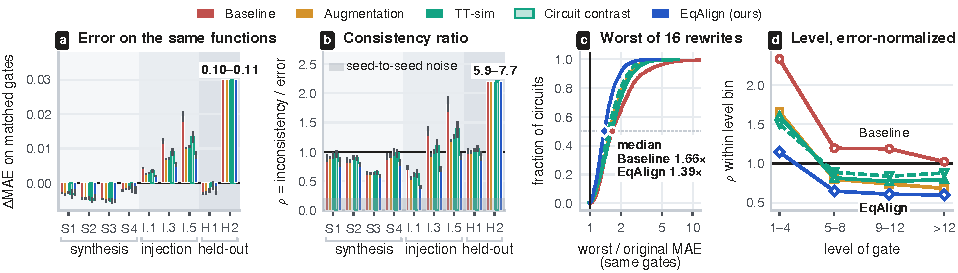
\includegraphics[width=0.92\textwidth]{figs/fig_audit.pdf}}\extonly{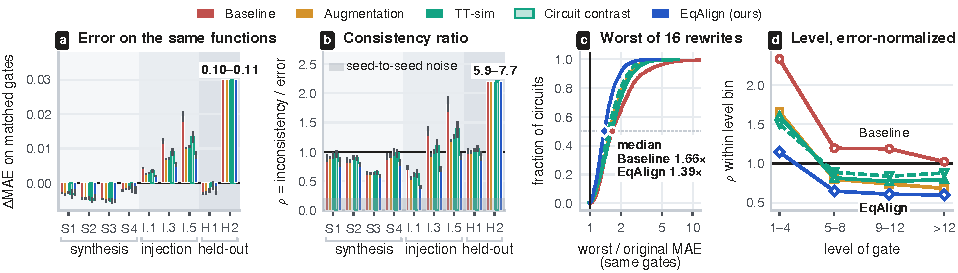
\includegraphics[width=\textwidth]{figs/fig_audit.pdf}}
\caption{\textbf{The audit on EPFL.} (a) Matched-gate degradation per family (H1, H2: held-out). (b)
Consistency ratio $\rho$; gray band: the baseline's seed-to-seed disagreement over its error (training
noise alone); H2 bars clipped, range above. (c) Per-circuit worst ratio over 16 adversarial variants. (d)
$\rho$ within level bins (7 fixed families). (a, b): mean $\pm$ s.d., (c, d): pooled, over 5 seeds.}
\label{fig:audit}
\end{figure*}}
\FigAudit

% ===========================================================================
\section{Experimental Setup}\label{sec:setup}
% ===========================================================================
\noindent\textbf{Data.} We extract random fanin cones from the EPFL combinational suite~\cite{epfl} and call each
cone a \emph{circuit} (\GatesMin\ to \GatesMax\ gates, test median \GatesMed; up to \InMax\ inputs). Training uses 11 designs\extonly{ (bar,
max, sin, multiplier, square, div, arbiter, mem\_ctrl, voter, i2c and priority)}; testing, the disjoint designs
log2, sqrt, adder, cavlc, ctrl, int2float and router (dec yields none); \extonly{dec yields no circuit, since each of its outputs is a
single 8-input minterm of 7 gates; }hyp, the largest
EPFL design, unused in development, is held back as a confirmatory design (\cref{sec:generality}). Of the \NTrainConesAll\ training circuits, \NValCones\ form a
validation split, and each training circuit is paired, in rotation, with one certified variant from S1 to S4 or injection at
$r\in\{0.15,0.3\}$. Each of the \NTestCones\ test circuits has 7 fixed, 2 held-out and 16 adversarial variants (two
circuits lack held-out ones\extonly{: the don't-care pass of H1 crashes on them, and it runs in the same process as H2}). A second, test-only suite of \ISCones\
circuits comes from ISCAS85 and ISCAS89's combinational cores (\cref{sec:generality}). Labels $p_v$ come
from 4{,}096 random input patterns shared by a circuit and its variants, so proven pairs share
labels.

\noindent\textbf{Training and selection.} All regimes use the same encoder, Adam with a one-cycle cosine
schedule (peak $2\!\times\!10^{-3}$, chosen from $\{2,1,0.5\}\!\times\!10^{-3}$ on the baseline's validation MAE), gradient clipping
at 1.0, 16-circuit batches, 12 epochs and 5 seeds, on GPUs (PyTorch~2.7).
Loss weights are chosen on validation by one rule, the highest restructured retrieval with validation MAE within
25\% of the baseline: $\lambda=\LamStar$\extonly{ from $\{0.05,0.1,0.2,0.5,1,2\}$}, $\lambda_{\mathrm{TT}}=\TTLamStar$\extonly{ from
$\{0.03,0.1,0.5,1,2\}$}, and $\lambda_{\mathrm C}=\CircLamStar$\extonly{ from $\{0.05,0.2,0.5,1\}$}\mainonly{ (grids in the extended version)}\extonly{; $L_1$ alignment takes $\LoneLam$ from
$\{0.0003,0.001,0.003,0.01,0.03\}$ and $L_1$ alignment + TT-sim $\LonettLam$ from $\{0.001,0.003,0.01\}$}. An exploratory version\extonly{ (constant learning rate, signature-only matching,
no projection)} saw the test designs before this protocol was fixed; every reported model was retrained under it, and
no test result entered selection or tuning.

\noindent\textbf{GPU and CPU runs.} Results come from this \emph{GPU run} unless marked. An earlier \emph{CPU run}
(PyTorch~2.15, 3 seeds), which the GPU run reproduces on 67 of 68 metrics with preset tolerances\extonly{ (\cref{app:repro})}, supplies only the
hyp results, \cref{fig:overview}'s pair, \cref{fig:sweep}b's timings, the solver test of \cref{sec:rq1} and the \extonly{released-model audits (Public rows of \cref{tab:general})}\mainonly{Public rows of \cref{tab:general}}.

\noindent\textbf{Statistics.} The EPFL test circuits come from 7 designs and overlap within a design,
so circuit-level tests would overstate significance. To compare two regimes we average each design over its
circuits and seeds, and report the mean difference with a 95\% cluster-bootstrap confidence interval (CI)
(${\ge}5{,}000$ design resamples~\cite{DBLP:books/sp/EfronT93}) and a two-sided sign test (smallest attainable $p$ with 7 EPFL
designs: 0.016; Holm-adjusted over regimes on the 17 ISCAS designs); for the 4 large-circuit designs (\cref{sec:generality}),
Holm-adjusted Welch tests over seeds.

% ===========================================================================
\section{Results}\label{sec:results}
% ===========================================================================
\extonly{\noindent Each subsection answers one research question (RQ1 to RQ4); \cref{tab:main,fig:audit} summarize the
audit of RQ1.}
% ===========================================================================


\subsection{RQ1: Is the Trained Model Equivalence Blind?}\label{sec:rq1}
\noindent\textbf{Under synthesis, accuracy holds but answers move.} On synthesis variants (\cref{tab:main}), the baseline is not
less accurate on matched gates ($\Delta$MAE $=\BaseDSyn$; matched gates get shallower, from level \DepthSynOrig\ to \DepthSynVar). Its
predictions still depend on the implementation: on restructured pairs, the two predictions for one function differ
by $\rho=\BaseRhoSyn$ times the model's error on those gates and by \IncSynOverNoiseBase\ times the seed
noise floor (\cref{fig:audit}b).\extonly{ Pooled over circuits, $\rho=\BaseRhoPoolSyn$, while an equally accurate model with independent errors on $v$ and
$u$ would have $\rho_\perp=\BaseRhoPerpSyn$: the baseline closes only $g=\BaseGapSyn\%$ of the gap to $\rho=0$.}

\noindent\textbf{Under redundancy, accuracy degrades.} Injection raises the matched-gate error by \BaseDInj\ and
$\rho$ to \BaseRhoInj, and the worst of 16 adversarial variants per circuit has \BaseWorstRatio$\times$ the original
error on those gates (ratio of means, \cref{fig:audit}c). Depth does not explain it: the baseline's $\rho$
exceeds 1 in every level bin (\cref{fig:audit}d).

\noindent\textbf{An unseen rewrite breaks every model.} On the held-out XOR-based rewrite H2, which adds reconvergent logic~\cite{DBLP:journals/tc/ParkerM75}, the
matched-gate error rises by about 0.1 and $\rho$ exceeds 5 for every regime (\cref{fig:audit}a,b). \extonly{A plausible
cause is reconvergence: $x\oplus y$ and $x\vee y$ share their inputs, and the probability of reconvergent logic
cannot be obtained by multiplying the probabilities of its dependent inputs~\cite{DBLP:journals/tc/ParkerM75}, a dependence absent
from training. }H1, built from passes similar to the training rewrites, stays near synthesis ($\rho\approx1$).

\noindent\textbf{Embeddings encode equivalence weakly.} The nearest original gate to a restructured
gate is its proven equivalent only \BaseTopRS\% of the time (chance \Chance\%), and proven pairs are separated
from same-level gates with AUROC$_\mathrm{lvl}$ \BaseAUCHard\ (chance 0.5).

\noindent\textbf{The blindness reaches decision rules.} Fed to CASCAD's phase rule~\cite{DBLP:journals/corr/abs-2508-04235} (fix a variable's phase if
$\hat p<0.01$ or $\hat p>0.99$; here on unconditional, not conditional, probabilities), the baseline fixes the phase in one
implementation of a function but not in the other for \DecFlipSyn\% of restructured pairs under synthesis, \DecRatioSyn\% as
often as it decides wrongly, and for \DecFlipHTwo\% under H2 against \DecErrHTwo\% wrong decisions. The 5\% of gates it predicts hardest
to activate overlap between a circuit and its synthesis, injection and H2 variants with Jaccard index \DecJacSyn, \DecJacInj\ and \DecJacHTwo\ (1 for
identical sets)\extonly{; \cref{app:decisions}}. In CaDiCaL (\PhInst\ bug-injected equivalence checks; CPU-run models), such static
hints add conflicts even from simulated probabilities (\PhOracleRatio$\times$), and matching a variant's hints to its proven
equivalents' does not reduce them (\PhSwapInv$\times$\extonly{; \cref{app:solver}}).

\begin{figure}[t]
\centering
\mainonly{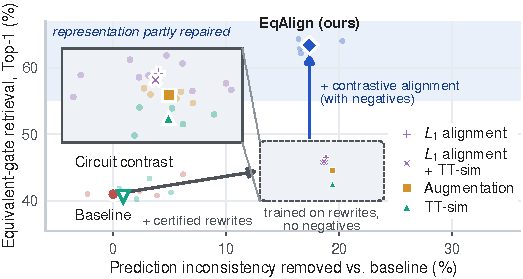
\includegraphics[width=0.9\columnwidth]{figs/fig_twolevel.pdf}}\extonly{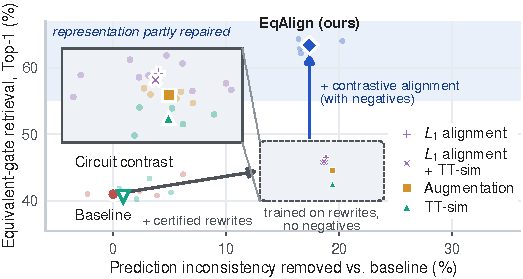
\includegraphics[width=\columnwidth]{figs/fig_twolevel.pdf}}
\caption{\textbf{Two levels of repair} on restructured pairs. \extonly{$x$: prediction inconsistency removed relative to the
baseline; $y$: Top-1 retrieval of the proven equivalent. }Small dots: seeds; large markers: 5-seed means. Inset: the
dashed box, \extonly{where every regime trained on rewrites without negatives lands (see key)}\mainonly{with every regime trained on rewrites without negatives}.}
\label{fig:twolevel}
\end{figure}


\subsection{RQ2: What Repairs It, and How Far Does the Repair Reach?}\label{sec:rq2}
\noindent\textbf{Augmentation repairs predictions, mainly under injection.} Training on certified variants lowers the
restructured inconsistency on all 7 test designs (design-level change \DTIncABDiff, 95\% CI
[\DTIncABLo,\,\DTIncABHi]) and $\rho$ under injection from \BaseRhoInj\ to \AugRhoInj, but leaves $\rho$ under synthesis
unchanged (\BaseRhoSyn\ and \AugRhoSyn), at no measurable accuracy
cost\extonly{ (MAE change \DTMaeABDiff, CI [\DTMaeABLo,\,\DTMaeABHi])}. Retrieval rises only from \BaseTopRS\% to \AugTopRS\%. Four variants per circuit instead of one add only
\EFourAugGainMin\ to \EFourAugGainMax\ points (state widths 64, 256), \EFourGapMin\ to \EFourGapMax\ below \ours\ with one\extonly{ (\cref{app:datascale})}. Representation losses without gate
correspondence fare no better (\extonly{TT-sim \TTTopRS\%, circuit-level contrast \CircTopRS\%}\mainonly{\cref{tab:main}}).


\extonly{\begin{table}[t]
\centering
\caption{\textbf{Loss weights and ablations} (seed 0); $\star$: the weight selected on validation by the rule fixed
in advance.\extonly{ The other weights of TT-sim ($\{0.5,1,2\}$) and circuit contrast (1) reach at most 33.3\% and 35.3\%
validation Top-1.}}
\label{tab:ablation}
\footnotesize\setlength{\tabcolsep}{3pt}
\resizebox{\columnwidth}{!}{\begin{tabular}{l cc cccc}
\toprule
 & \multicolumn{2}{c}{Validation} & \multicolumn{4}{c}{Test (seen families)} \\
\cmidrule(lr){2-3}\cmidrule(lr){4-7}
Variant & MAE & Top-1 & MAE & $\rho$ & Top-1 & AUROC$_\mathrm{lvl}$ \\
\midrule
Baseline & 0.0148 & 33.9 & 0.0189 & 0.97 & 41.5 & 0.766 \\
Augmentation & 0.0152 & 36.8 & 0.0177 & 0.86 & 44.8 & 0.785 \\
\midrule
\ours\ $\lambda$=0.05 & 0.0145 & 53.7 & 0.0183 & 0.80 & 61.6 & 0.856 \\
\ours\ $\lambda$=0.1 & 0.0151 & 57.0 & 0.0191 & 0.81 & 62.5 & 0.838 \\
\ours\ $\lambda$=0.2$^\star$ & 0.0166 & 58.7 & 0.0228 & 0.70 & 62.2 & 0.844 \\
\ours\ $\lambda$=0.5 & 0.0192 & 58.3 & 0.0258 & 0.72 & 60.9 & 0.858 \\
\ours\ no proj., $\lambda$=0.2 & 0.0161 & 55.9 & 0.0244 & 0.85 & 59.6 & 0.831 \\
\midrule
TT-sim $\lambda_{\mathrm{TT}}$=0.03$^\star$ & 0.0150 & 34.9 & 0.0171 & 0.94 & 40.9 & 0.768 \\
Circuit contrast $\lambda_{\mathrm{C}}$=0.2$^\star$ & 0.0167 & 39.1 & 0.0186 & 0.97 & 41.3 & 0.821 \\
\bottomrule
\end{tabular}
}
\end{table}}
\noindent\textbf{\ours\ partly repairs the representation on seen rewrites.} \ours\ raises restructured retrieval to
\OursTopRS\% (\cref{fig:twolevel}) and AUROC$_\mathrm{lvl}$ to \OursAUCHard, with the lowest $\rho$ in every column of \cref{tab:main}, partly because it errs more. The gap closed $g$
still favors it under injection (\OursGapInj\% against \BaseGapInj\% to \AugGapInj\% for the regimes of
\cref{tab:main}, on all 7 designs) but not under synthesis\extonly{ (all regimes close \BaseGapSyn\% to \OursGapSyn\%, with no
consistent difference across designs)}, where it repairs where equivalent gates sit, not what they predict.
At design level it beats the baseline by \DTTopOBDiff\ points (CI [\DTTopOBLo,\,\DTTopOBHi]) and
augmentation, TT-sim and circuit-level contrast by \DTTopOADiff, \DTTopOTDiff\ and \DTTopOCDiff\extonly{ (augmentation CI
[\DTTopOALo,\,\DTTopOAHi])}, each on all 7 designs (\extonly{each sign test $p=\DTTopOBP$; }all intervals above 0\extonly{; Welch tests over seeds against all six other regimes, Holm-adjusted: $p<\WelchHolmTopMax$}).
Simulation does better: 64-pattern signatures alone retrieve \SigRefSixtyFour\% of these pairs. \ours\ costs accuracy on original circuits: its MAE is
\OursMAECostPct\% above the baseline's (design level: \DTMaeOBDiff, CI [\DTMaeOBLo,\,\DTMaeOBHi], not significant) and
\OursMAECostAugPct\% above that of augmentation, which sees the same variants. The cost is tunable: $\lambda=0.05$
keeps baseline-level MAE at \LowLamTop\% retrieval (seed 0)\extonly{ (\cref{tab:ablation})}, and the projection head adds \NoHeadDiff\ points
(CI [\NoHeadLo,\,\NoHeadHi]).

% Fig. 4 is defined here so that it opens the right column of the page where RQ3 cites it
\begin{figure}[t]
\centering
\mainonly{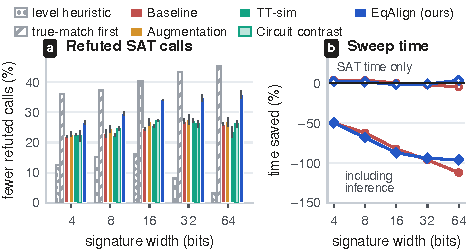
\includegraphics[width=0.92\columnwidth]{figs/fig_sweep.pdf}}\extonly{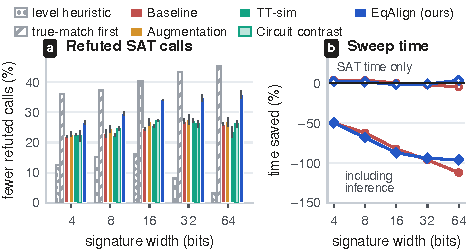
\includegraphics[width=\columnwidth]{figs/fig_sweep.pdf}}
\caption{\textbf{SAT-sweeping probe} (\extonly{5 designs $\times$ 4 variants, }pooled per seed; mean and s.e.\ over 3
seeds: GPU run in (a), CPU run in (b)). (a) Fewer refuted SAT calls than topological order; outlined: non-learned orders, filled: embeddings of
the model of that color. (b) Change in sweep time, SAT only (open) and with \extonly{embedding inference on one CPU core}\mainonly{inference} (filled).}
\label{fig:sweep}
\end{figure}
\noindent\textbf{Alignment without negatives repairs only the predictions.} \emph{$L_1$ alignment},
MixGate's loss~\cite{DBLP:journals/corr/abs-2509-20968} on our proven pairs with the weight chosen by the same rule, reaches \LoneTop\% retrieval
(\emph{$L_1$ alignment + TT-sim}: \LonettTop\%), close to augmentation's \AugTopRS\%, and the same inconsistency\extonly{;
larger weights collapse the embeddings}. Positives-only cosine alignment through the same head
retrieves \EightCosTop\%, below \ours\ on all 7 designs\extonly{ (5 seeds; \EightWDiff\ at width 256)}: here, telling
equivalent gates apart needs negatives.

\noindent\textbf{The gain needs gate correspondence and encoder training; proofs serve measurement.} Training only the projection head, with the same loss and pairs, on a frozen encoder reaches \ProbeBaseTop\% on the
baseline encoder and \ProbeAugTop\% on the augmented one: \EncShare\% of the gain over the baseline requires changing
the encoder, so it is not a readout effect\extonly{; retrieval on the encoder state instead of the projection gives
\HretTop\%}. Replacing the proven pairs by pairs matched on 4{,}096-bit or 64-bit
simulation signatures gives \SigFourKTop\% and \SigSixtyFourTop\%. The loss needs correspondences, which simulation
supplies cheaply; proofs matter for measurement.

\noindent\textbf{Repair transfers within a kind of rewrite, not across kinds, and coverage has a price.} Trained
without one synthesis script (3 seeds, widths 64 and 256; design-level means), \ours\ loses at most \TwSynCostMax\ points on it and still beats
augmentation there by \TwSynVsAugMin\ to \TwSynVsAugMax; never trained on ABC, it raises retrieval under ABC's scripts as much as
under ours (\AbcBaseTop\% to \AbcOursTop\% against \AbcBaseTopSyn\% to \AbcOursTopSyn\%), most on dc2 (\AbcBaseTopDc\% to \AbcOursTopDc\%), and in
fine-tuned DeepGate2 (\AbcFtCtrlTop\% with its own loss, \AbcFtEqTop\% with \ours); trained without injection, it retrieves \TwInjOurs\% of injected pairs
(\TwInjFull\% with them), below augmentation's \TwInjAug\% on every design\extonly{ (width 256: \TwWInjOurs\%, \TwWInjFull\% and
\TwWInjAug\%), while its retrieval under synthesis rises by \TwOthGain\ and \TwWOthGain\ points}. H2\extonly{, on which every regime
fails (\cref{tab:main}; \ours\ retrieves \OursTopHo\% on the held-out families, the baseline \BaseTopHo\%),} is
learnable: over 5 seeds, adding H2 variants to training lifts \ours's H2 retrieval from \NineEqHTwoBefore\% to
\NineEqHTwoAfter\%\extonly{ (error increase \NineEqDHTwoBefore\ to \NineEqDHTwoAfter)}, but its seen-rewrite retrieval falls from
\NineEqSeenBefore\% to \NineEqSeenAfter\% on every design and its MAE rises by \NineEqMaePct\%, at width 256 too\extonly{ (\NineEqWSeenBefore\% to \NineEqWSeenAfter\%, design-level change
\NineEqWSeenDiff\ points, CI [\NineEqWSeenLo,\,\NineEqWSeenHi]; at width 64 \NineEqSeenDiff, CI [\NineEqSeenLo,\,\NineEqSeenHi]),
and augmentation pays it too (seen retrieval \NineAugSeenBefore\% to \NineAugSeenAfter\%)}. Certified data repair the
rewrites they contain, not equivalence, and adding H2 costs invariance to the seen ones.



\subsection{RQ3: Do Aligned Embeddings Help SAT Sweeping?}\label{sec:rq3}
\noindent\textbf{The signal is real but does not pay here.} We sweep five full EPFL test designs (\extonly{ctrl, router, int2float, cavlc, adder; }174 to 1{,}020 gates) against four
certified variants each (\cref{fig:sweep})\extonly{: for every variant gate, original gates with matching $k$-bit signatures are candidates,
refined by SAT counterexamples and tried in a given order until one is proven}. Candidate orders differ only in refuted SAT
calls; the reference is topological order, as in fraiging. With 8-bit
signatures, ordering by \ours\ embeddings removes \SwOursEmbEight\% of refuted calls, against \SwBaseEmbEight\% for
baseline embeddings, \SwLevelEight\% for a logic-level heuristic and \SwTrueEight\% for trying the true match first%
\extonly{ (64-bit: \SwOursEmbSixtyFour\%, \SwBaseEmbSixtyFour\%, \SwLevelSixtyFour\%, \SwTrueSixtyFour\%)}. Here,
refuted calls on designs this small are cheap, so SAT time changes
by only \SwCpuSatTimeEight\%, while embedding inference slows the sweep at 8 bits by \SwCpuSlowEight\%
on one CPU core (\SwCpuEmbMs\,ms per circuit pair)\extonly{, and by \SwOursEmbSlowEight\% on the GPU machine, shared with training
jobs (\SwEmbMs\,ms)}. RQ3 measures equivalence information, not
DeepGate2's industrial-scale speed-up~\cite{DBLP:conf/iccad/ShiPKLLHZYCX23}.


\subsection{RQ4: Do the Findings Generalize Beyond Our Setup?}\label{sec:generality}
\newcommand{\TabGeneral}{%
\begin{table}[t]
\centering
\caption{\textbf{Generality} (seed means\extonly{; \cref{sec:generality}}). ISCAS: EPFL-trained; \extonly{$w$: state width; }\mainonly{$w$: width; }Bidir., Transf.: Top-1 over all pairs;
DG2: DeepGate2; FT: fine-tuned; $^\dagger$GPU run; --: no prob.\ head; H.-o.: \extonly{mean of H1, H2}\mainonly{held-out}\extonly{; EPFL Top-1 chance:
\DTwoChance\%}.}
\label{tab:general}
\footnotesize\setlength{\tabcolsep}{1.9pt}
\begin{tabular}{ll c ccc c cc}
\toprule
 & & MAE$\downarrow$ & \multicolumn{3}{c}{$\rho\downarrow$} & $\Delta$MAE$\downarrow$ & \multicolumn{2}{c}{Top-1 (\%)$\uparrow$} \\
\cmidrule(lr){4-6}\cmidrule(lr){7-7}\cmidrule(lr){8-9}
Setting & Model & orig. & Syn. & Inj. & H.-o. & H.-o. & seen & H.-o. \\
\midrule
\multirow{5}{*}{ISCAS} & \mk{cbase}\ Baseline & 0.0353 & 0.86 & 0.81 & 2.49 & \textbf{0.0395} & 27.0 & 14.4 \\
 & \mk{caug}\ Augmentation & \textbf{0.0332} & 0.83 & 0.56 & 2.62 & 0.0414 & 29.7 & 15.7 \\
 & \mk{ctt}\ TT-sim & 0.0333 & \textbf{0.82} & 0.55 & 2.60 & 0.0410 & 28.7 & 15.3 \\
 & \mk{ccirc}\ Circuit contrast & 0.0343 & 0.88 & 0.69 & \textbf{2.47} & 0.0409 & 29.8 & 17.3 \\
 & \hl \mk{cours}\ \ours & \hl 0.0340 & \hl \textbf{0.82} & \hl \textbf{0.50} & \hl \textbf{2.47} & \hl 0.0414 & \hl \textbf{41.8} & \hl \textbf{23.3} \\
\midrule
\multirow{3}{*}{\shortstack[l]{Bidir.\\$w{=}64$}} & \mk{cbase}\ Baseline & 0.0183 & 0.71 & 1.23 & 3.70 & 0.0509 & 49.4 & 31.9 \\
 & \mk{caug}\ Augmentation & \textbf{0.0170} & 0.70 & 0.85 & 3.88 & 0.0519 & 50.9 & 32.5 \\
 & \hl \mk{cours}\ \ours & \hl 0.0203 & \hl \textbf{0.66} & \hl \textbf{0.74} & \hl \textbf{3.35} & \hl \textbf{0.0505} & \hl \textbf{78.5} & \hl \textbf{51.4} \\
\midrule
\multirow{3}{*}{\shortstack[l]{Transf.\\$w{=}128$}} & \mk{cbase}\ Baseline & 0.0197 & 0.76 & 1.23 & \textbf{3.42} & \textbf{0.0503} & 17.5 & 12.6 \\
 & \mk{caug}\ Augmentation & \textbf{0.0184} & 0.69 & 0.81 & 3.66 & 0.0520 & 18.8 & 13.5 \\
 & \hl \mk{cours}\ \ours & \hl 0.0190 & \hl \textbf{0.68} & \hl \textbf{0.62} & \hl 3.52 & \hl 0.0517 & \hl \textbf{49.0} & \hl \textbf{31.8} \\
\midrule
\multirow{6}{*}{\shortstack[l]{Public\\(CPU)}} & DeepGate2 & 0.0287 & 0.63 & 1.01 & 2.54 & 0.0468 & 37.4 & 22.6 \\
 & DG2 retrained$^\dagger$ & 0.0479 & 0.51 & 0.75 & 1.69 & 0.0446 & 35.3 & 22.3 \\
 & DG3 tokenizer & 0.0214 & 0.85 & 1.34 & 3.82 & 0.0510 & 42.9 & 28.5 \\
 & FGNN2 & -- & -- & -- & -- & -- & 61.9 & 43.5 \\
 & MGVGA & -- & -- & -- & -- & -- & 20.4 & 12.7 \\
 & TRACE & -- & -- & -- & -- & -- & 66.6 & 43.6 \\
\midrule
\multirow{2}{*}{\shortstack[l]{FT\\(GPU)}} & DG2 + own loss & \textbf{0.0269} & \textbf{0.66} & 0.78 & 2.80 & 0.0501 & 40.1 & 23.6 \\
 & \hl \mk{cours}\ DG2 + \ours & \hl 0.0322 & \hl 0.68 & \hl \textbf{0.63} & \hl \textbf{2.29} & \hl \textbf{0.0465} & \hl \textbf{66.6} & \hl \textbf{39.2} \\
\bottomrule
\end{tabular}

\end{table}}
\mainonly{\TabGeneral}
\noindent\textbf{Confirmatory design.} With all other results fixed, we evaluated the 15 CPU-run models
(5 regimes, 3 seeds) on \HypCones\ hyp circuits\extonly{; the 25 GPU models,
evaluated later, agree (\ours\ \HypGpuOursTop\% against at most \HypGpuBestOtherTop\%, its worst seed \HypGpuOursTopMin\% above every other
regime's best, \HypGpuOtherTopMax\%)}. The main findings replicate: the baseline's $\rho$ under
synthesis is \HypBaseRhoSyn, augmentation lowers $\rho$ under injection (\HypBaseRhoInj\ to \HypAugRhoInj), H2 raises every
regime's matched-gate error by \HypHTwoMin\ to \HypHTwoMax, and \ours\ retrieves \HypOursTop\% against at most
\HypBestOtherTop\% otherwise\extonly{ (worst \ours\ seed \HypOursTopMin\%, best
other \HypOtherTopMax\%). Two secondary findings do not: \ours's AUROC$_\mathrm{lvl}$ (\HypOursAUC) does not exceed the other
representation losses' (up to \HypBestOtherAUC), and it pays no accuracy cost there (MAE \HypOursMAE, the lowest)}.

\extonly{\TabGeneral}
\noindent\textbf{Second benchmark suite.} On ISCAS85/89, with EPFL-trained models, synthesis moves
baseline predictions\extonly{ by $\rho=\ISBaseRhoSyn$}, H2 breaks every regime, and \ours\ raises retrieval\extonly{ from
\ISBaseTopRS\% to \ISOursTopRS\%}, beyond every other regime\extonly{ tested} on all \IsDesN\ designs (\extonly{design-level gaps \IsDesTopMin\ to \IsDesTopMax\ points, }Holm-adjusted
sign test $p<10^{-4}$; \cref{tab:general}).

\noindent\textbf{ABC synthesis scripts.} Under ABC's scripts, all \AbcNArch\ baseline encoders (3 architectures, 3 widths each) stay blind ($\rho$ \AbcAllRhoMin\ to \AbcAllRhoMax, against
\AbcAllRhoSynMin\ to \AbcAllRhoSynMax\ under ours; released DeepGate2: \AbcDTwoRho) with no rise in matched-gate error; augmentation does
not lower the inconsistency (all intervals include 0), and the recurrent \ours\ beats every regime on all 7 designs at width 64
and on all but ctrl (16 cones) at width 256 (gains: \cref{sec:rq2})\extonly{; on ISCAS it raises retrieval from \AbcIsBaseTop\% to \AbcIsOursTop\%, and in fine-tuned DeepGate2 from
\AbcIsFtCtrlTop\% to \AbcIsFtEqTop\% (\cref{app:abc})}.

\noindent\textbf{Other architectures.} A bidirectional encoder (attention, reverse pass)
and a transformer show the two levels at every width tested (64 to 512): \ours\ raises retrieval\extonly{ over all
proven pairs from \BiBaseTopRS\% to \BiOursTopRS\% and from \TfBaseTopRS\% to \TfOursTopRS\%}\mainonly{ (\cref{tab:general})}, beyond every other regime\extonly{ tested} on all 7
designs, and all fail on H2\extonly{; augmentation lowers $\rho$ under injection from \BiBaseRhoInj\ to \BiAugRhoInj\ and
from \TfBaseRhoInj\ to \TfAugRhoInj\ (all widths: \cref{tab:app_arch})}.

\noindent\textbf{Released checkpoints.} We ran \audit\ unchanged on the functional embedding $\mathbf h_f$ of released
DeepGate2 and the DeepGate3 tokenizer (released without its refining transformer); both were trained on
subcircuits that include EPFL designs~\cite{DBLP:conf/iccad/ShiPKLLHZYCX23,DBLP:conf/iccad/ShiZKZ0024}. \extonly{Both draw fresh random primary-input vectors per
forward pass, so the same circuit retrieves only \DTwoSelfRand\% and \DThreeSelfRand\% of its own gates; we share
them across a rewrite, which changes no conclusion. }Both show the pattern (\cref{tab:general}): \extonly{re-synthesis moves the prediction
for a fixed function by \DTwoRhoSyn\ and \DThreeRhoSyn\ times the model's error, and the held-out families take
retrieval from \DTwoTopSeen\% and \DThreeTopSeen\% to \DTwoTopHo\% and \DThreeTopHo\%}\mainonly{predictions move under re-synthesis and retrieval falls under held-out families} (H2 alone: \DTwoHTwoRS\% and \DThreeHTwoRS\%). Retrained with its released code and data
(\TenSeeds\ seeds), DeepGate2 errs more than its released weights\extonly{ (MAE \TenMAE\ vs.\ \TenRelMAE)} yet disagrees nearly as much (\TenIncons\ vs.\ \TenRelIncons) and fails alike (\extonly{\TenTop\% seen, }\TenHTwo\% under H2): blindness
is not specific to one checkpoint, and higher accuracy did not reduce it\extonly{ (its lower
$\rho$ in \cref{tab:general} reflects the larger error in the denominator, not a smaller disagreement)}.\extonly{ From DeepGate2 to DeepGate3's tokenizer, the restructured error falls by
\DThreeErrDrop\% but the disagreement across a rewrite by only \DThreeInconsDrop\%.}

\noindent\textbf{Released gate-state encoders.} TRACE, MGVGA and FGNN2~\cite{DBLP:conf/dac/ZhengZZX26,DBLP:conf/iclr/WuZ0025,DBLP:journals/tcad/WangBHZXHHY25} have no
probability head; we audit their gate states\extonly{, with input conventions fixed by each model's own pretraining
objective (\cref{app:ext})}. TRACE and FGNN2, trained for equivalence, retrieve
\extonly{\TrSeen\% and \FgSeen\% on seen rewrites, the most of any released encoder,}\mainonly{the most of any released encoder on seen rewrites (\cref{tab:general})} but \TrHTwo\% and \FgHTwo\% under H2;
MGVGA, which gives many gates identical embeddings (\MgSelf\% retrieval within an identical copy), gets \extonly{\MgSeen\% and \MgHTwo\% (H2)}\mainonly{\MgHTwo\% under H2}.

\noindent\textbf{Repairing a released model.} Fine-tuning released DeepGate2 on our training data
(5 epochs, \FtEqSeeds\ seeds) with its own loss moves retrieval from \TenRelTop\% (released weights, GPU evaluation) to \FtCtrlTopSeen\%; adding \ours\ on $\mathbf h_f$
reaches \FtEqTopSeen\% (higher on all 7 designs\extonly{, design-level gain \FtDiff\ points}\extonly{, CI [\FtDiffLo,\,\FtDiffHi]}; held-out \FtEqTopHo\% vs.\
\FtCtrlTopHo\%) at \FtMaeCostPct\% higher MAE.

\noindent\textbf{Model and circuit size.} Growing the encoder \ScFold-fold (recurrent widths 64 to 1024, \ScMinParams\ to
\ScMaxParams\ parameters, and 4 instead of 2 passes; transformers 128 to 512) leaves blindness intact: the recurrent baseline's $\rho$ under synthesis
stays between \ScBaseRhoMin\ and \ScBaseRhoMax\ and its retrieval drifts from \ScBaseTopFirst\% to \ScBaseTopLast\%, while \ours\ leads the
baseline and augmentation by \ScLeadMin\ to \ScLeadMax\ design-level points at every size, on all 7 designs\extonly{ (5 seeds each; at width
256 it leads every regime by \WDiffMin\ to \WDiffMax\ points, and synthesis inconsistency is \WNoise\ times the seed noise floor;
all sizes: \cref{tab:app_scale})}. On \LgCones\ test circuits of \LgGatesMin\ to \LgGatesMax\ gates (median \LgGatesMed) from \LgDesigns\ arithmetic
designs, retrieval falls for every regime as candidates multiply (chance \LgChance\%): the baseline retrieves
\LgBaseTop\%, \ours\ \LgOursTop\%, above every other regime (at most \LgOtherMax\%) on all \LgDesigns\ designs (Welch $p<10^{-4}$\extonly{, Holm-adjusted; too few designs for a design-level test}); none exceeds \LgHTwoMax\% under H2\extonly{; width 256 gives \LgWBaseTop\%, \LgWOursTop\% and at most \LgWOtherMax\%}.

% ===========================================================================
% Extended version: a full Threats to Validity section; the 7-page version states its limitations at the end of the
% Conclusion instead (a section heading there would cost the space the limitations need).
\extonly{
\section{Threats to Validity}\label{sec:limits}
\noindent\textbf{Task.} Signal probability is the only function-level prediction we audit, and SAT sweeping and
CASCAD's phase rule (also given to CaDiCaL, \cref{app:solver}) are the only downstream uses we probe; other tasks may show other degrees of blindness. The audit
itself does not depend on the task: any per-gate prediction or embedding can be compared across certified variants.
\textbf{Rewrites.} Training synthesis comes from one library (mockturtle, through aigverse); four ABC scripts test transfer
to another tool (\cref{app:abc}), and commercial flows may restructure differently. Injection is a stress test, not a realistic flow, so every family is reported separately.
\textbf{Circuits.} All circuits are combinational AIGs; ISCAS89 enters through its combinational cores. Training circuits
have under 400 gates and swept designs at most 1{,}020; larger test circuits are those certified within \LgTimeoutMin\
minutes (\LgTimeout\ of \LgBuilt\ timed out), and on them \ours's MAE exceeds the baseline's by \LgMaePct\%, beyond our
25\% tolerance. \textbf{Scale.} Our largest encoder has \ScMaxParams\ parameters; beyond our own encoders we audit only the
five published checkpoints of \cref{tab:general}. \textbf{Labels.} Signal probabilities assume uniform
inputs and carry sampling noise of about $10^{-2}$, on which inconsistency does not depend. \textbf{Statistics.} Seven
EPFL test designs bound the design-level sign test at $p\ge0.016$; we therefore report intervals and per-design counts,
and confirm on the 17 ISCAS designs and on hyp, which no stage of development used but which is a single design
(\HypCones\ circuits). \textbf{Retrieval.} Matching records the first proven equivalent of each variant gate, so a
different but equivalent nearest gate counts as a miss (\cref{app:matching}); reported retrieval is a lower bound.
\textbf{Released checkpoints.} We share the random primary-input vectors of DeepGate2 and DeepGate3 across a rewrite; this
raises some retrievals by about 5 points and changes no conclusion (\cref{app:pi}). \textbf{GPU and CPU runs.} The GPU run
reproduces the CPU run on 67 of 68 comparable metrics (\cref{app:repro}); each result names its run.
\textbf{Selection.} Learning rate and loss weights are chosen on validation circuits of the training designs only, and
picks at the edge of a grid are reported, not re-tuned.
}
% ===========================================================================
\section{Conclusion}
% ===========================================================================
With SAT proofs of equivalence, \audit\ makes the premise of circuit representation learning testable: a
function-trained encoder changes its answer for a fixed function by about as much as it errs. Among our regimes, certified data and
alignment without negatives steady the predictions, only contrastive alignment of matched gates partly repairs the
representation, and none survives an unseen kind of rewrite.

\mainonly{\noindent\textbf{Limitations.} We audit one function-level task, signal probability, with two downstream probes;
other tasks may differ. Synthesis comes from mockturtle and ABC, and injection is a stress test, not a realistic flow.
Training circuits have under 400 gates, swept designs at most 1{,}020, and our largest encoder \ScMaxParams\ parameters;
larger test circuits are those certified within \LgTimeoutMin\ minutes (\LgTimeout\ of \LgBuilt\ timed out), and on them
\ours's MAE exceeds the baseline's by \LgMaePct\%, beyond our 25\% tolerance. Seven EPFL test designs bound the sign
test at $p\ge0.016$, so ISCAS and hyp carry the confirmation (\cref{sec:generality}).}

\mainonly{\noindent}We propose certified equivalence as a standard check; the held-out failure motivates encoders
invariant by construction.

% Camera-ready: the Acknowledgment section goes here (removed for blind review).
\section*{Content Generated by AI}
The authors used Claude Opus 5.5 to assist with copyediting, grammar checking, and the retouching and fine refinement of all figures in the paper. The authors take full
responsibility for the accuracy and integrity of this paper.
